\documentclass[12pt,a4paper]{article}

\usepackage{fontspec}
\usepackage[russian]{babel}
\usepackage{amsmath, amssymb}
\usepackage{geometry}
\usepackage{graphicx}
\usepackage{booktabs}
\usepackage{array}
\usepackage{float}
\usepackage{caption}
\usepackage{hyperref}
\usepackage{listings}
\usepackage{xcolor}

\setmainfont{Times New Roman}
\setsansfont{Arial}
\setmonofont{Menlo}

\geometry{margin=2cm}
\setlength{\parindent}{1.25cm}
\setlength{\parskip}{0.35em}

\lstset{
    basicstyle=\ttfamily\small,
    breaklines=true,
    frame=single,
    columns=fullflexible,
    keepspaces=true,
    extendedchars=true
}

\begin{document}

\begin{titlepage}
    \begin{center}
        Федеральное государственное автономное образовательное учреждение\\
        высшего образования\\
        <<Национальный исследовательский университет ИТМО>>

        \vspace*{0.28\textheight}

        {\Large \textbf{Отчёт}}\\
        {\large \textbf{По лабораторной работе №5}}\\
        {\large по дисциплине <<Вычислительная математика>>}\\
        {\large \textbf{Вариант: 4}}
    \end{center}

    \vfill

    \begin{flushright}
        Студент:\\
        Красноштанова Юлия Николаевна\\
        Группа Р3216\\
        Преподаватель:\\
        Наумова Надежда Александровна
    \end{flushright}

    \vfill

    \begin{center}
        г. Санкт-Петербург 2026
    \end{center}
\end{titlepage}

\section*{Цель работы}
Решить задачу интерполяции: найти значения функции при заданных значениях аргумента, отличных от узловых точек.

\section*{Задание}
\begin{enumerate}
    \item Выбрать из таблицы вариантов заданную таблицу $y=f(x)$ (таблица 1.4).
    \item Построить таблицу конечных разностей для заданной таблицы.
    \item Вычислить значение функции для аргумента $X_1$, используя первую или вторую интерполяционную формулу Ньютона.
    \item Вычислить значение функции для аргумента $X_2$, используя первую или вторую интерполяционную формулу Гаусса.
    \item Вычислить значения функции для аргументов $X_1$ и $X_2$ с помощью многочлена Лагранжа.
    \item Предусмотреть ввод исходных данных тремя способами: таблицей с клавиатуры, из файла (не менее трёх тестовых вариантов) и на основе функции $f(x)$, выражение которой вводится с клавиатуры, с заданием отрезка и числа узлов.
    \item Сформировать и вывести таблицу конечных и разделённых разностей.
    \item Вычислить приближённое значение функции для введённого с клавиатуры аргумента методами по варианту: многочлен Лагранжа, многочлен Ньютона с разделёнными разностями (1 и 2 формулы), многочлен Ньютона с конечными разностями (1 и 2 формулы). Сравнить полученные значения.
    \item Построить графики заданной функции с отмеченными узлами интерполяции и интерполяционного многочлена.
    \item Протестировать программу при различных наборах данных, в том числе некорректных.
\end{enumerate}

\section*{Рабочие формулы}
Пусть функция задана таблицей узлов $(x_i;y_i)$, $i=0,1,\ldots,n$, причём все $x_i$ различны. Требуется построить многочлен $P_n(x)$ степени не выше $n$, удовлетворяющий условиям интерполяции $P_n(x_i)=y_i$, и вычислить его значение в точке $x$, отличной от узлов. Такой многочлен единственен, поэтому все рассмотренные ниже формулы дают одно и то же значение и отличаются только способом вычисления.

\subsection*{Многочлен Лагранжа}
\[
    L_n(x)=\sum_{i=0}^{n}y_i\,l_i(x),\qquad
    l_i(x)=\prod_{\substack{j=0\\ j\ne i}}^{n}\frac{x-x_j}{x_i-x_j}.
\]
Базисный многочлен $l_i(x)$ равен единице в узле $x_i$ и нулю во всех остальных узлах. Формула применима при любом расположении узлов.

\subsection*{Многочлен Ньютона с разделёнными разностями}
Разделённые разности нулевого порядка совпадают со значениями функции $f(x_i)=y_i$, разности первого и следующих порядков определяются рекуррентно:
\[
    f(x_i,x_{i+1})=\frac{f(x_{i+1})-f(x_i)}{x_{i+1}-x_i},\qquad
    f(x_i,\ldots,x_{i+k})=\frac{f(x_{i+1},\ldots,x_{i+k})-f(x_i,\ldots,x_{i+k-1})}{x_{i+k}-x_i}.
\]
Первая интерполяционная формула Ньютона (вперёд):
\[
\begin{aligned}
    N_n(x)&=f(x_0)+f(x_0,x_1)(x-x_0)+f(x_0,x_1,x_2)(x-x_0)(x-x_1)+\ldots\\
    &\quad+f(x_0,\ldots,x_n)(x-x_0)(x-x_1)\cdots(x-x_{n-1}).
\end{aligned}
\]
Вторая интерполяционная формула Ньютона (назад):
\[
\begin{aligned}
    N_n(x)&=f(x_n)+f(x_{n-1},x_n)(x-x_n)+f(x_{n-2},x_{n-1},x_n)(x-x_n)(x-x_{n-1})+\ldots\\
    &\quad+f(x_0,\ldots,x_n)(x-x_n)(x-x_{n-1})\cdots(x-x_1).
\end{aligned}
\]
Первая формула используется для точек левой половины отрезка $[x_0;x_n]$, вторая -- для правой. Узлы могут быть неравноотстоящими.

\subsection*{Многочлен Ньютона с конечными разностями}
Для равноотстоящих узлов $x_i=x_0+ih$ вводятся конечные разности
\[
    \Delta y_i=y_{i+1}-y_i,\qquad \Delta^k y_i=\Delta^{k-1}y_{i+1}-\Delta^{k-1}y_i .
\]
Первая интерполяционная формула Ньютона (вперёд), $t=\dfrac{x-x_0}{h}$:
\[
    N_n(x)=y_0+t\,\Delta y_0+\frac{t(t-1)}{2!}\Delta^2y_0+\ldots+\frac{t(t-1)\cdots(t-n+1)}{n!}\Delta^ny_0 .
\]
Вторая интерполяционная формула Ньютона (назад), $t=\dfrac{x-x_n}{h}$:
\[
    N_n(x)=y_n+t\,\Delta y_{n-1}+\frac{t(t+1)}{2!}\Delta^2y_{n-2}+\ldots+\frac{t(t+1)\cdots(t+n-1)}{n!}\Delta^ny_0 .
\]
Первая формула применяется в левой половине отрезка (и для экстраполирования при $x<x_0$), вторая -- в правой половине (и при $x>x_n$).

\subsection*{Интерполяционные формулы Гаусса}
Для интерполирования в середине таблицы узлы нумеруются относительно центрального узла $a=x_0$: $x_{\pm k}=a\pm kh$, $t=\dfrac{x-a}{h}$.
Первая формула Гаусса ($x>a$, $t>0$):
\[
    P_n(x)=y_0+t\,\Delta y_0+\frac{t(t-1)}{2!}\Delta^2y_{-1}+\frac{(t+1)t(t-1)}{3!}\Delta^3y_{-1}+\frac{(t+1)t(t-1)(t-2)}{4!}\Delta^4y_{-2}+\ldots
\]
Вторая формула Гаусса ($x<a$, $t<0$):
\[
    P_n(x)=y_0+t\,\Delta y_{-1}+\frac{t(t+1)}{2!}\Delta^2y_{-1}+\frac{(t+1)t(t-1)}{3!}\Delta^3y_{-2}+\frac{(t+2)(t+1)t(t-1)}{4!}\Delta^4y_{-2}+\ldots
\]
В обеих формулах используются разности, ближайшие к центральной строке таблицы.

\section*{Вычислительная часть}
Для варианта 4 задана таблица 1.4 из семи равноотстоящих узлов с шагом $h=0{,}1$ и точки $X_1=1{,}051$, $X_2=1{,}277$.

\begin{table}[H]
    \centering
    \caption{Исходная таблица варианта 4}
    \begin{tabular}{l*{7}{c}}
        \toprule
        $x_i$ & $1{,}05$ & $1{,}15$ & $1{,}25$ & $1{,}35$ & $1{,}45$ & $1{,}55$ & $1{,}65$\\
        $y_i$ & $0{,}1213$ & $1{,}1316$ & $2{,}1459$ & $3{,}1565$ & $4{,}1571$ & $5{,}1819$ & $6{,}1969$\\
        \bottomrule
    \end{tabular}
\end{table}

\subsection*{Таблица конечных разностей}
Конечные разности вычисляются по формуле $\Delta^k y_i=\Delta^{k-1}y_{i+1}-\Delta^{k-1}y_i$, например $\Delta y_0=1{,}1316-0{,}1213=1{,}0103$, $\Delta^2y_0=1{,}0143-1{,}0103=0{,}0040$.

\begin{table}[H]
    \centering
    \footnotesize
    \setlength{\tabcolsep}{4pt}
    \caption{Таблица конечных разностей}
    \begin{tabular}{ccccccccc}
        \toprule
        $i$ & $x_i$ & $y_i$ & $\Delta y_i$ & $\Delta^2y_i$ & $\Delta^3y_i$ & $\Delta^4y_i$ & $\Delta^5y_i$ & $\Delta^6y_i$\\
        \midrule
        0 & $1{,}05$ & $0{,}1213$ & $1{,}0103$ & $0{,}0040$ & $-0{,}0077$ & $0{,}0014$ & $0{,}0391$ & $-0{,}1478$\\
        1 & $1{,}15$ & $1{,}1316$ & $1{,}0143$ & $-0{,}0037$ & $-0{,}0063$ & $0{,}0405$ & $-0{,}1087$ & \\
        2 & $1{,}25$ & $2{,}1459$ & $1{,}0106$ & $-0{,}0100$ & $0{,}0342$ & $-0{,}0682$ & & \\
        3 & $1{,}35$ & $3{,}1565$ & $1{,}0006$ & $0{,}0242$ & $-0{,}0340$ & & & \\
        4 & $1{,}45$ & $4{,}1571$ & $1{,}0248$ & $-0{,}0098$ & & & & \\
        5 & $1{,}55$ & $5{,}1819$ & $1{,}0150$ & & & & & \\
        6 & $1{,}65$ & $6{,}1969$ & & & & & & \\
        \bottomrule
    \end{tabular}
\end{table}

\subsection*{Значение в точке $X_1$ по формуле Ньютона}
Точка $X_1=1{,}051$ лежит в начале таблицы (левая половина отрезка), поэтому используется первая интерполяционная формула Ньютона с разностями $\Delta^ky_0$ из верхней строки таблицы:
\[
    t=\frac{X_1-x_0}{h}=\frac{1{,}051-1{,}05}{0{,}1}=0{,}01 .
\]
\[
\begin{aligned}
    N_6(X_1)&=y_0+t\,\Delta y_0+\frac{t(t-1)}{2!}\Delta^2y_0+\frac{t(t-1)(t-2)}{3!}\Delta^3y_0+\frac{t(t-1)(t-2)(t-3)}{4!}\Delta^4y_0\\
    &\quad+\frac{t(t-1)(t-2)(t-3)(t-4)}{5!}\Delta^5y_0+\frac{t(t-1)(t-2)(t-3)(t-4)(t-5)}{6!}\Delta^6y_0 .
\end{aligned}
\]
Множители при разностях:
\[
\begin{aligned}
    t&=0{,}01,\\
    \frac{t(t-1)}{2!}&=\frac{0{,}01\cdot(-0{,}99)}{2}=-0{,}00495,\\
    \frac{t(t-1)(t-2)}{3!}&=\frac{0{,}01\cdot(-0{,}99)\cdot(-1{,}99)}{6}=0{,}0032835,\\
    \frac{t(t-1)(t-2)(t-3)}{4!}&=\frac{0{,}01\cdot(-0{,}99)\cdot(-1{,}99)\cdot(-2{,}99)}{24}=-0{,}0024544,\\
    \frac{t(t-1)(t-2)(t-3)(t-4)}{5!}&=\frac{0{,}01\cdot(-0{,}99)\cdots(-3{,}99)}{120}=0{,}0019586,\\
    \frac{t(t-1)(t-2)(t-3)(t-4)(t-5)}{6!}&=\frac{0{,}01\cdot(-0{,}99)\cdots(-4{,}99)}{720}=-0{,}0016289 .
\end{aligned}
\]
Слагаемые:
\[
\begin{aligned}
    N_6(X_1)&=0{,}1213+0{,}01\cdot1{,}0103-0{,}00495\cdot0{,}0040+0{,}0032835\cdot(-0{,}0077)\\
    &\quad-0{,}0024544\cdot0{,}0014+0{,}0019586\cdot0{,}0391-0{,}0016289\cdot(-0{,}1478)\\
    &=0{,}1213+0{,}010103-0{,}0000198-0{,}0000253-0{,}0000034+0{,}0000766+0{,}0002408\\
    &=0{,}131672 .
\end{aligned}
\]
Основной вклад даёт линейный член, поправки высших порядков малы, так как $t$ близко к нулю.

\subsection*{Значение в точке $X_2$ по формуле Гаусса}
Точка $X_2=1{,}277$ находится в середине таблицы. За центральный узел принимаем средний узел таблицы $a=x_3=1{,}35$ -- при таком выборе в формуле можно использовать все разности вплоть до $\Delta^6y$. В центральной нумерации $y_0=3{,}1565$, $y_{-1}=2{,}1459$, $y_{-2}=1{,}1316$, $y_{-3}=0{,}1213$, и
\[
    t=\frac{X_2-a}{h}=\frac{1{,}277-1{,}35}{0{,}1}=-0{,}73<0,
\]
поэтому применяется вторая интерполяционная формула Гаусса:
\[
\begin{aligned}
    P_6(X_2)&=y_0+t\,\Delta y_{-1}+\frac{t(t+1)}{2!}\Delta^2y_{-1}+\frac{(t+1)t(t-1)}{3!}\Delta^3y_{-2}+\frac{(t+2)(t+1)t(t-1)}{4!}\Delta^4y_{-2}\\
    &\quad+\frac{(t+2)(t+1)t(t-1)(t-2)}{5!}\Delta^5y_{-3}+\frac{(t+3)(t+2)(t+1)t(t-1)(t-2)}{6!}\Delta^6y_{-3} .
\end{aligned}
\]
Нужные разности берутся из таблицы конечных разностей: $\Delta y_{-1}=\Delta y_2=1{,}0106$, $\Delta^2y_{-1}=\Delta^2y_2=-0{,}0100$, $\Delta^3y_{-2}=\Delta^3y_1=-0{,}0063$, $\Delta^4y_{-2}=\Delta^4y_1=0{,}0405$, $\Delta^5y_{-3}=\Delta^5y_0=0{,}0391$, $\Delta^6y_{-3}=\Delta^6y_0=-0{,}1478$.

Множители при разностях:
\[
\begin{aligned}
    t&=-0{,}73,\\
    \frac{t(t+1)}{2!}&=\frac{-0{,}73\cdot0{,}27}{2}=-0{,}09855,\\
    \frac{(t+1)t(t-1)}{3!}&=\frac{0{,}27\cdot(-0{,}73)\cdot(-1{,}73)}{6}=0{,}0568305,\\
    \frac{(t+2)(t+1)t(t-1)}{4!}&=\frac{1{,}27\cdot0{,}27\cdot(-0{,}73)\cdot(-1{,}73)}{24}=0{,}0180437,\\
    \frac{(t+2)(t+1)t(t-1)(t-2)}{5!}&=\frac{1{,}27\cdot0{,}27\cdot(-0{,}73)\cdots(-2{,}73)}{120}=-0{,}0098519,\\
    \frac{(t+3)(t+2)(t+1)t(t-1)(t-2)}{6!}&=\frac{2{,}27\cdot1{,}27\cdot0{,}27\cdots(-2{,}73)}{720}=-0{,}0037273 .
\end{aligned}
\]
Слагаемые:
\[
\begin{aligned}
    P_6(X_2)&=3{,}1565-0{,}73\cdot1{,}0106-0{,}09855\cdot(-0{,}0100)+0{,}0568305\cdot(-0{,}0063)\\
    &\quad+0{,}0180437\cdot0{,}0405-0{,}0098519\cdot0{,}0391-0{,}0037273\cdot(-0{,}1478)\\
    &=3{,}1565-0{,}737738+0{,}000986-0{,}000358+0{,}000731-0{,}000385+0{,}000551\\
    &=2{,}420287 .
\end{aligned}
\]

\subsection*{Значения в точках $X_1$ и $X_2$ по многочлену Лагранжа}
По семи узлам строится многочлен $L_6(x)=\sum_{i=0}^{6}y_i\,l_i(x)$. Значения базисных многочленов в точках $X_1$ и $X_2$ и слагаемые суммы приведены в таблице; например,
\[
    l_0(X_1)=\frac{(1{,}051-1{,}15)(1{,}051-1{,}25)\cdots(1{,}051-1{,}65)}{(1{,}05-1{,}15)(1{,}05-1{,}25)\cdots(1{,}05-1{,}65)}=0{,}975725 .
\]

\begin{table}[H]
    \centering
    \caption{Слагаемые многочлена Лагранжа}
    \begin{tabular}{cccccc}
        \toprule
        $i$ & $y_i$ & $l_i(X_1)$ & $y_i\,l_i(X_1)$ & $l_i(X_2)$ & $y_i\,l_i(X_2)$\\
        \midrule
        0 & $0{,}1213$ & $0{,}975725$ & $0{,}118355$ & $0{,}006125$ & $0{,}000743$\\
        1 & $1{,}1316$ & $0{,}059135$ & $0{,}066917$ & $-0{,}065682$ & $-0{,}074326$\\
        2 & $2{,}1459$ & $-0{,}073547$ & $-0{,}157825$ & $0{,}772376$ & $1{,}657442$\\
        3 & $3{,}1565$ & $0{,}065266$ & $0{,}206012$ & $0{,}380898$ & $1{,}202304$\\
        4 & $4{,}1571$ & $-0{,}036681$ & $-0{,}152488$ & $-0{,}120544$ & $-0{,}501114$\\
        5 & $5{,}1819$ & $0{,}011732$ & $0{,}060795$ & $0{,}030556$ & $0{,}158336$\\
        6 & $6{,}1969$ & $-0{,}001629$ & $-0{,}010094$ & $-0{,}003727$ & $-0{,}023098$\\
        \midrule
        \multicolumn{3}{r}{$L_6(X_1)=$} & $0{,}131672$ & $L_6(X_2)=$ & $2{,}420287$\\
        \bottomrule
    \end{tabular}
\end{table}

\begin{table}[H]
    \centering
    \caption{Сравнение результатов вычислительной части}
    \begin{tabular}{lcc}
        \toprule
        Метод & $X_1=1{,}051$ & $X_2=1{,}277$\\
        \midrule
        Первая формула Ньютона ($t=0{,}01$) & $0{,}131672$ & --\\
        Вторая формула Гаусса ($t=-0{,}73$) & -- & $2{,}420287$\\
        Многочлен Лагранжа & $0{,}131672$ & $2{,}420287$\\
        \bottomrule
    \end{tabular}
\end{table}

\textbf{Вывод по вычислительной части.} Значения, полученные разными формулами, совпадают: $y(1{,}051)\approx0{,}13167$ и $y(1{,}277)\approx2{,}42029$. Это объясняется единственностью интерполяционного многочлена степени 6 по семи узлам: формулы Ньютона, Гаусса и Лагранжа -- лишь разные способы записи одного многочлена. Для $X_1$ удобна первая формула Ньютона (точка у левого края таблицы), для $X_2$ -- вторая формула Гаусса (точка в середине таблицы левее центрального узла).

\section*{Графики}
На рисунке приведены узлы интерполяции варианта 4, интерполяционный многочлен и точки $X_1$, $X_2$.

\begin{figure}[H]
    \centering
    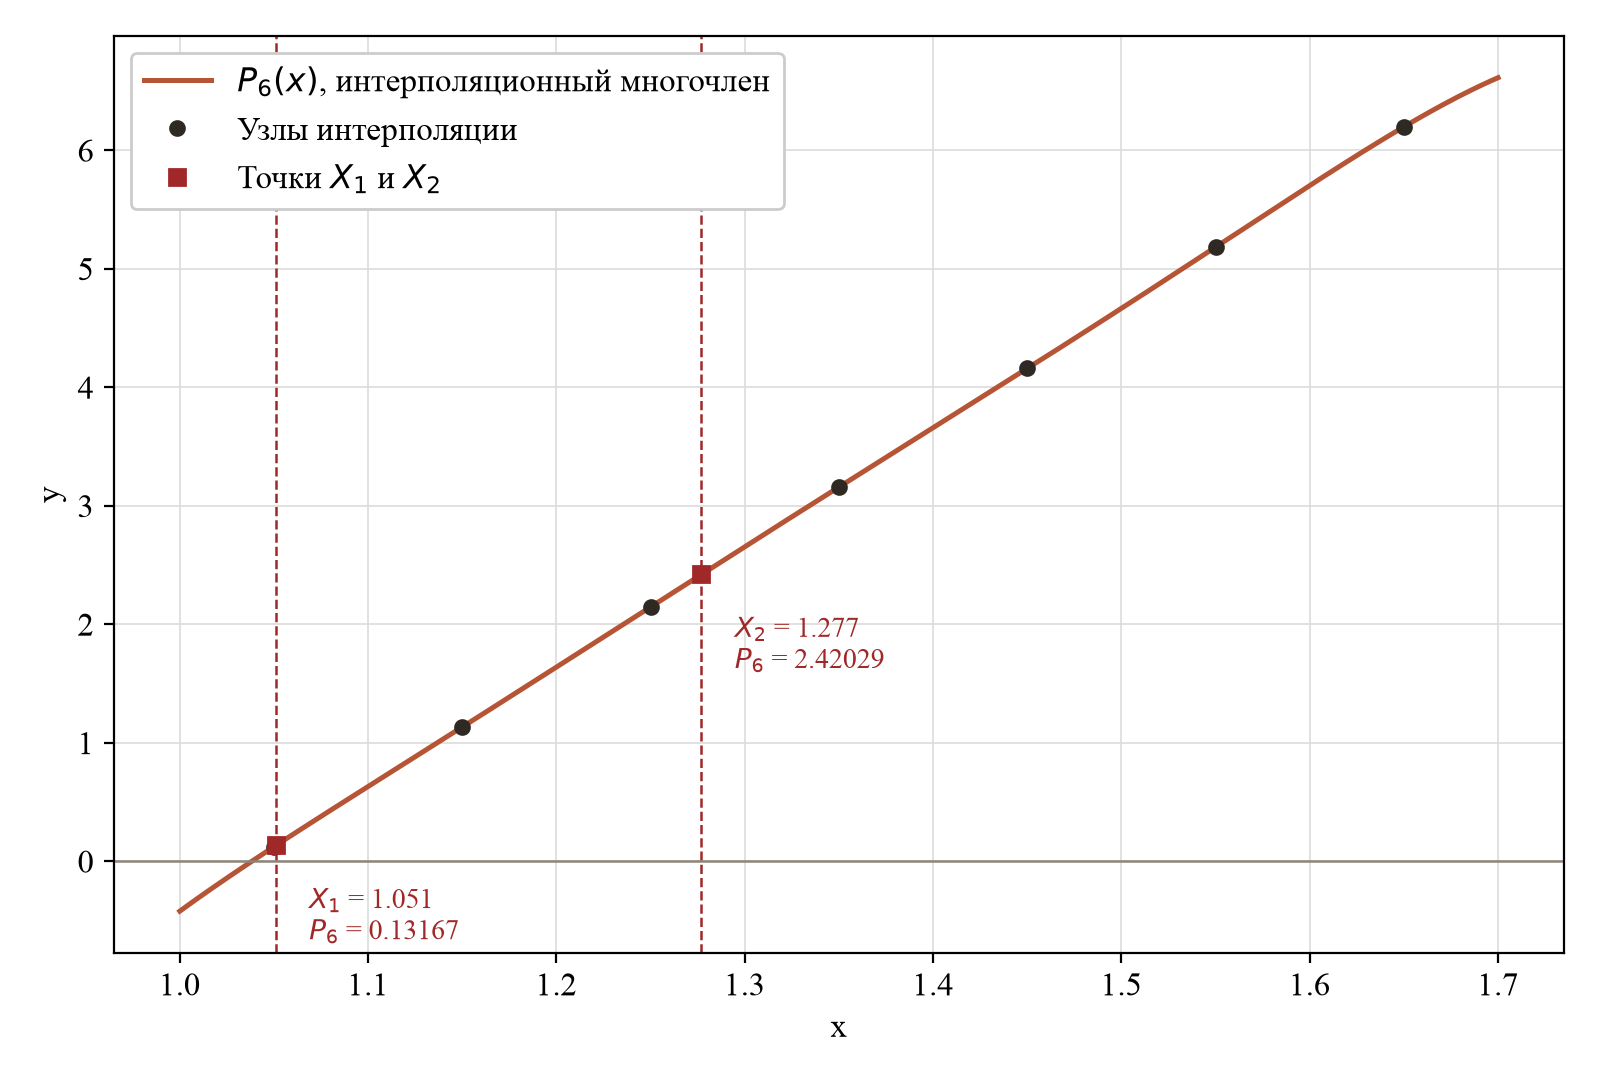
\includegraphics[width=\textwidth]{report_assets/computational_plot.png}
    \caption{Узлы интерполяции и интерполяционный многочлен варианта 4}
\end{figure}

Те же данные в программе: кривые трёх методов совпадают, точка $x=1{,}051$ отмечена вертикальной линией.

\begin{figure}[H]
    \centering
    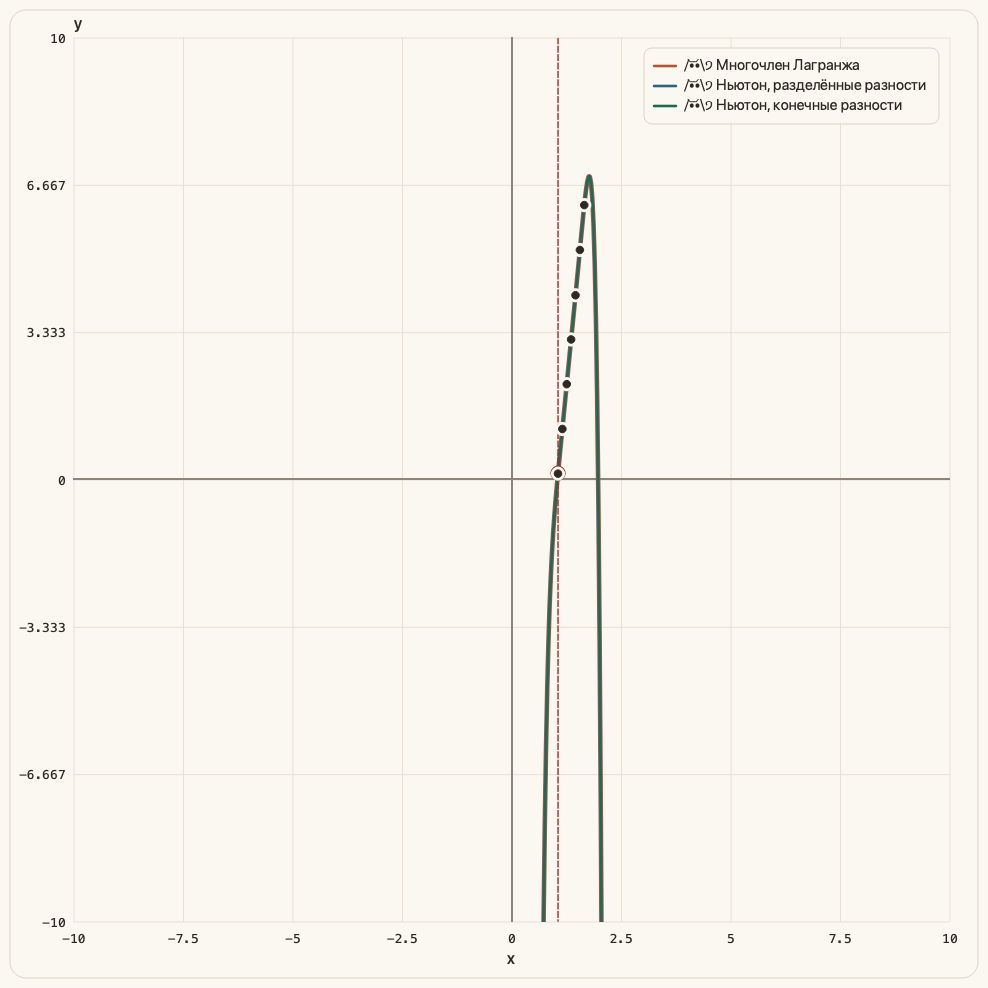
\includegraphics[width=0.85\textwidth]{report_assets/plot_variant4.png}
    \caption{Интерполяционные многочлены, построенные программой}
\end{figure}

\section*{Блок-схемы реализованных алгоритмов}
Блок-схемы построены по коду программы.

\begin{figure}[H]
    \centering
    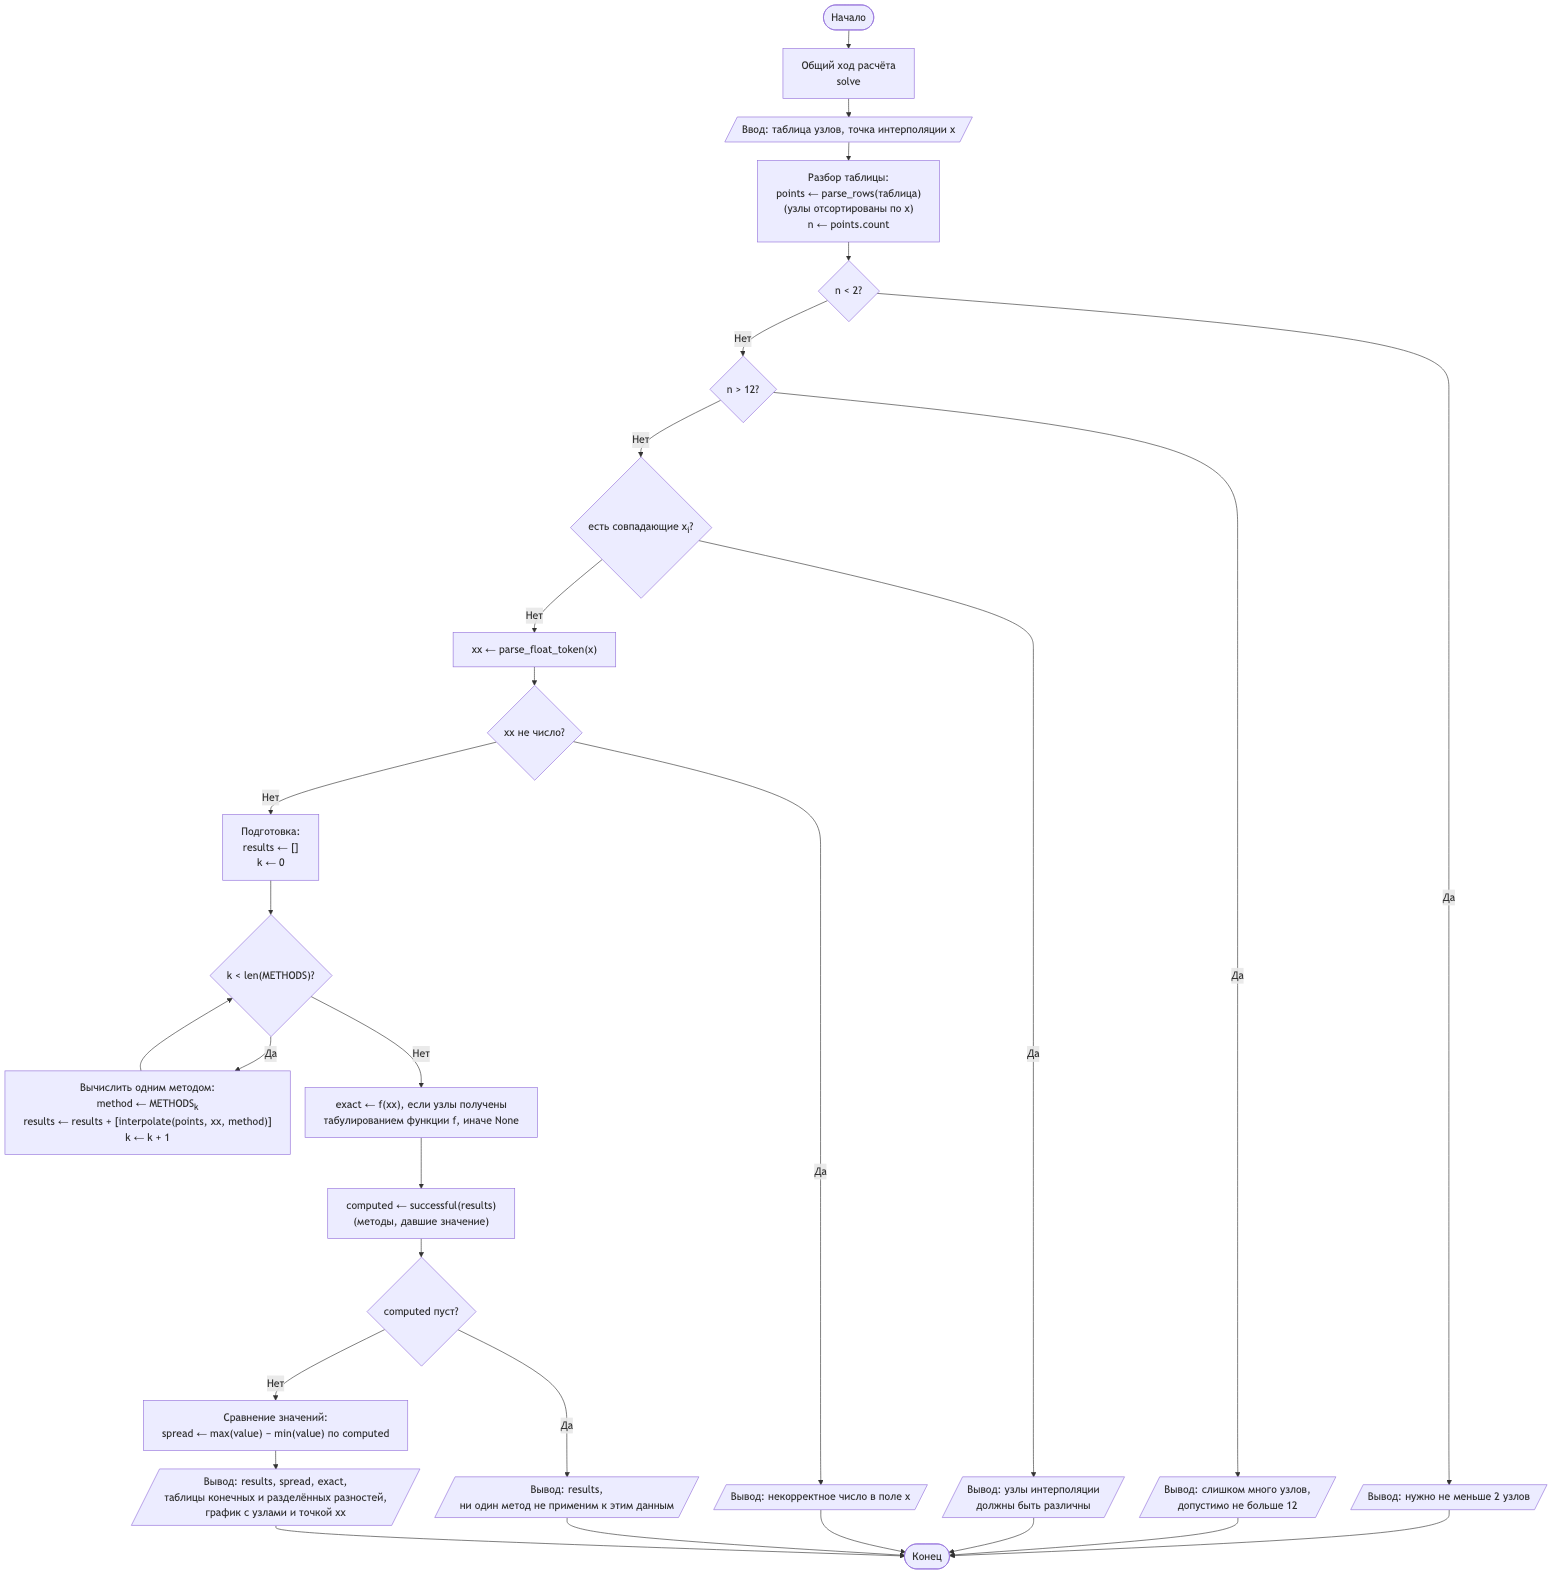
\includegraphics[width=\textwidth,height=0.82\textheight,keepaspectratio]{report_assets/solve.png}
    \caption{Блок-схема общего хода расчёта (функция \texttt{solve})}
\end{figure}

\begin{figure}[H]
    \centering
    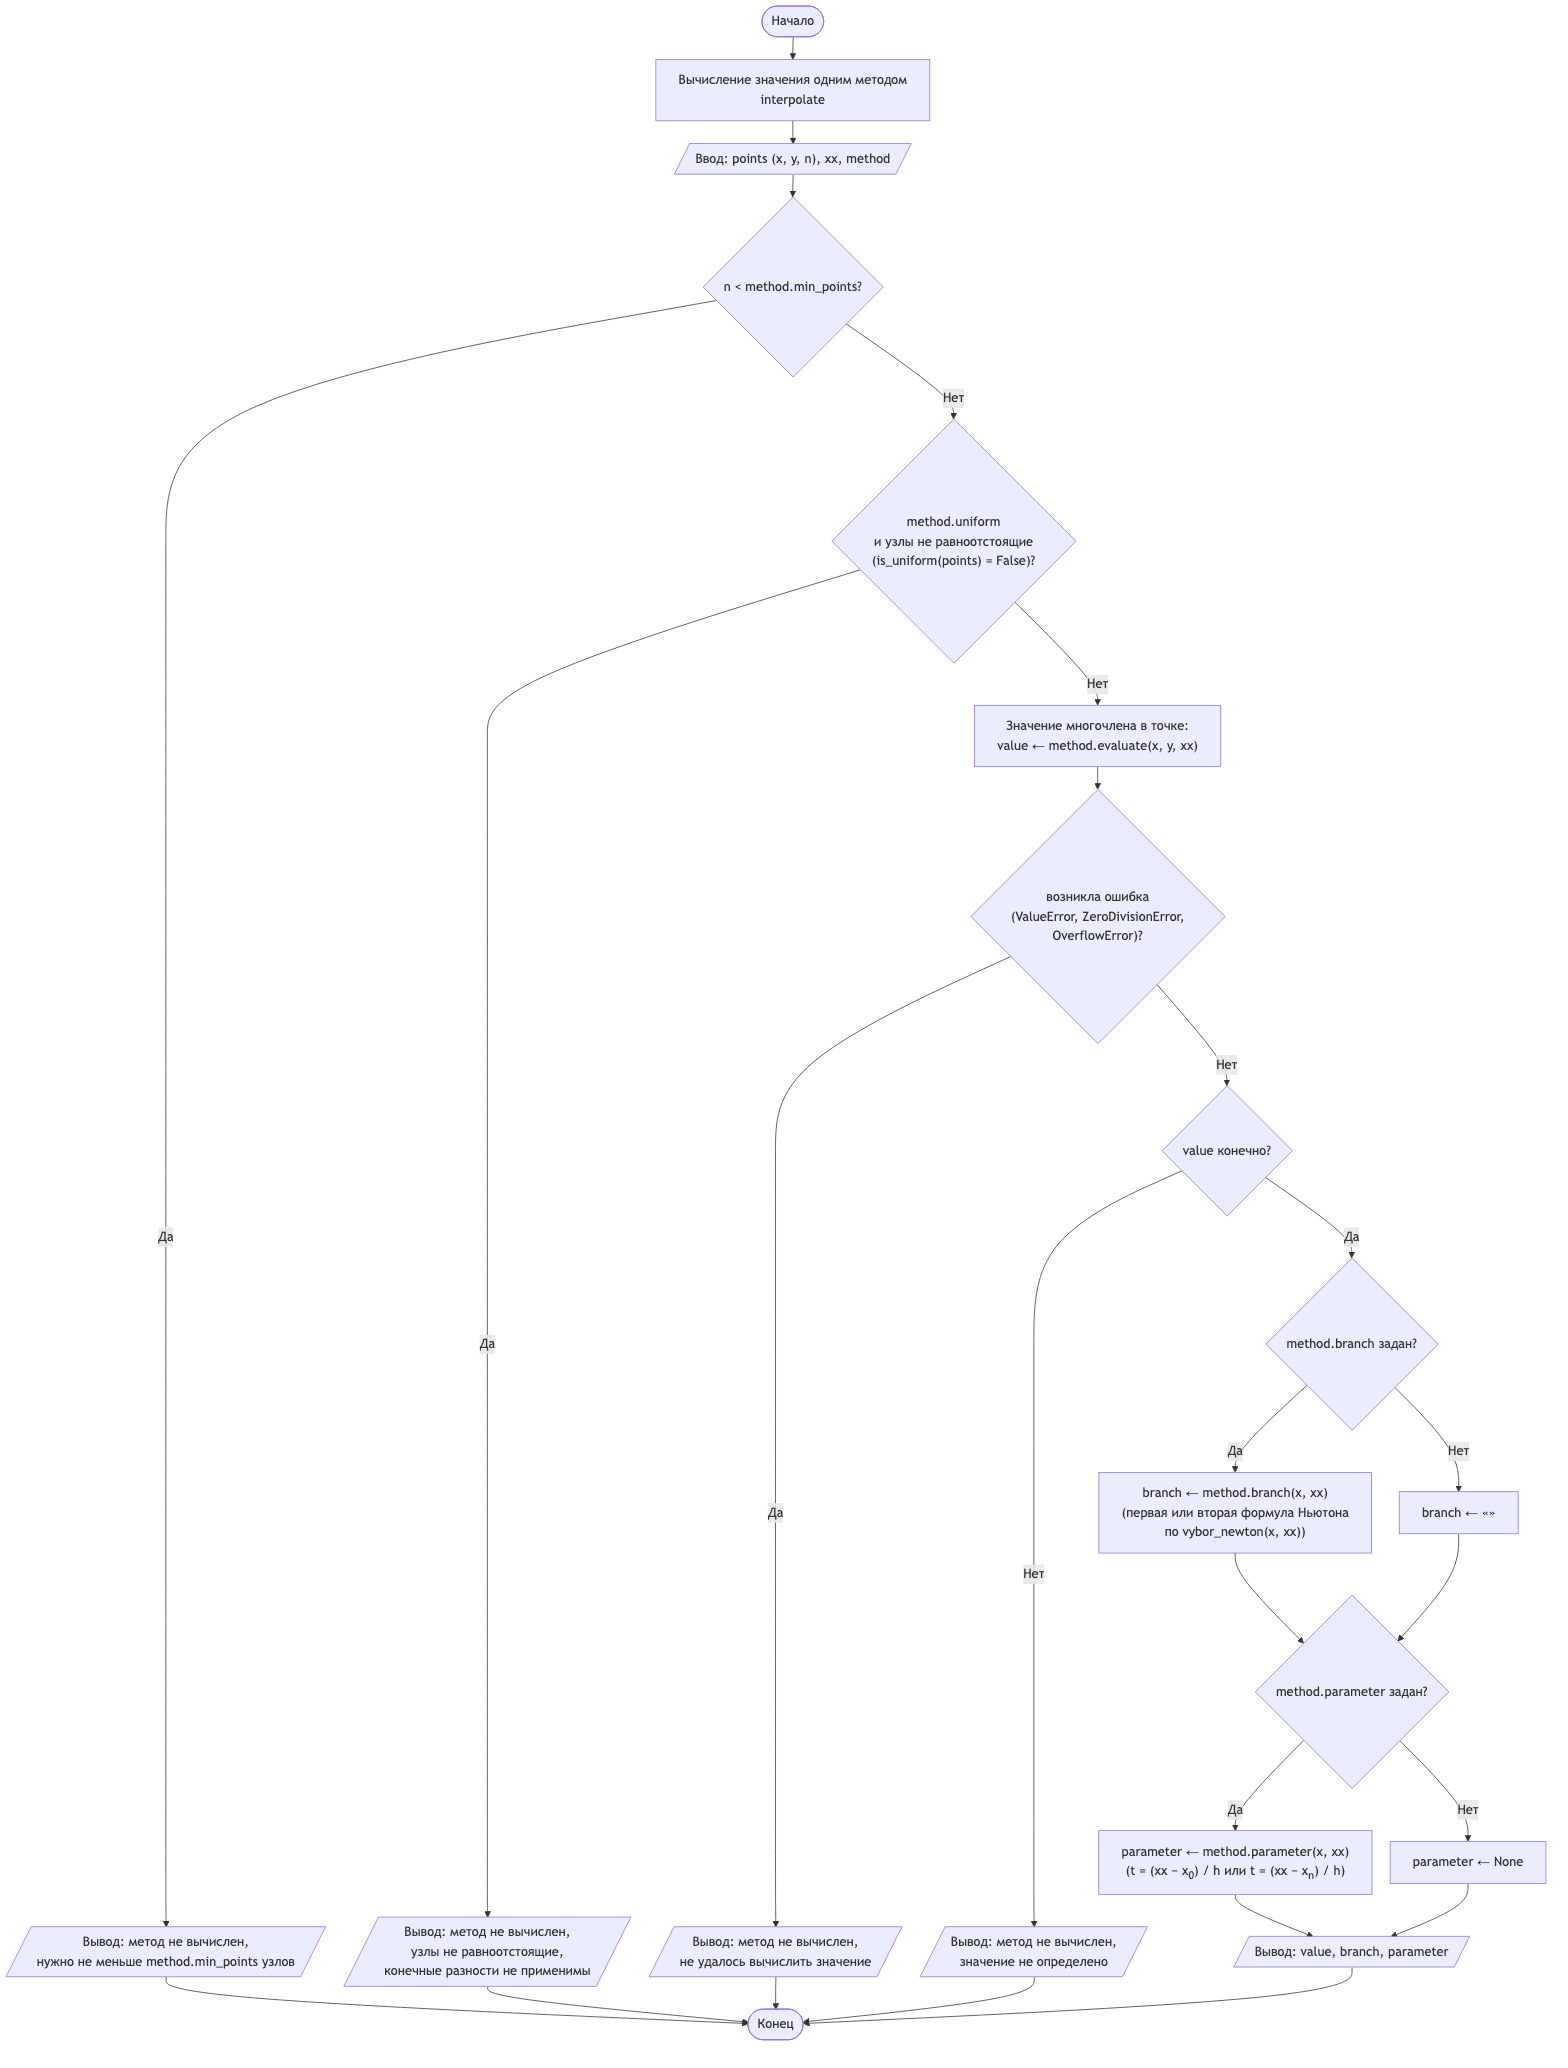
\includegraphics[width=\textwidth,height=0.82\textheight,keepaspectratio]{report_assets/interpolate.png}
    \caption{Блок-схема вычисления значения одним методом (функция \texttt{interpolate})}
\end{figure}

\begin{figure}[H]
    \centering
    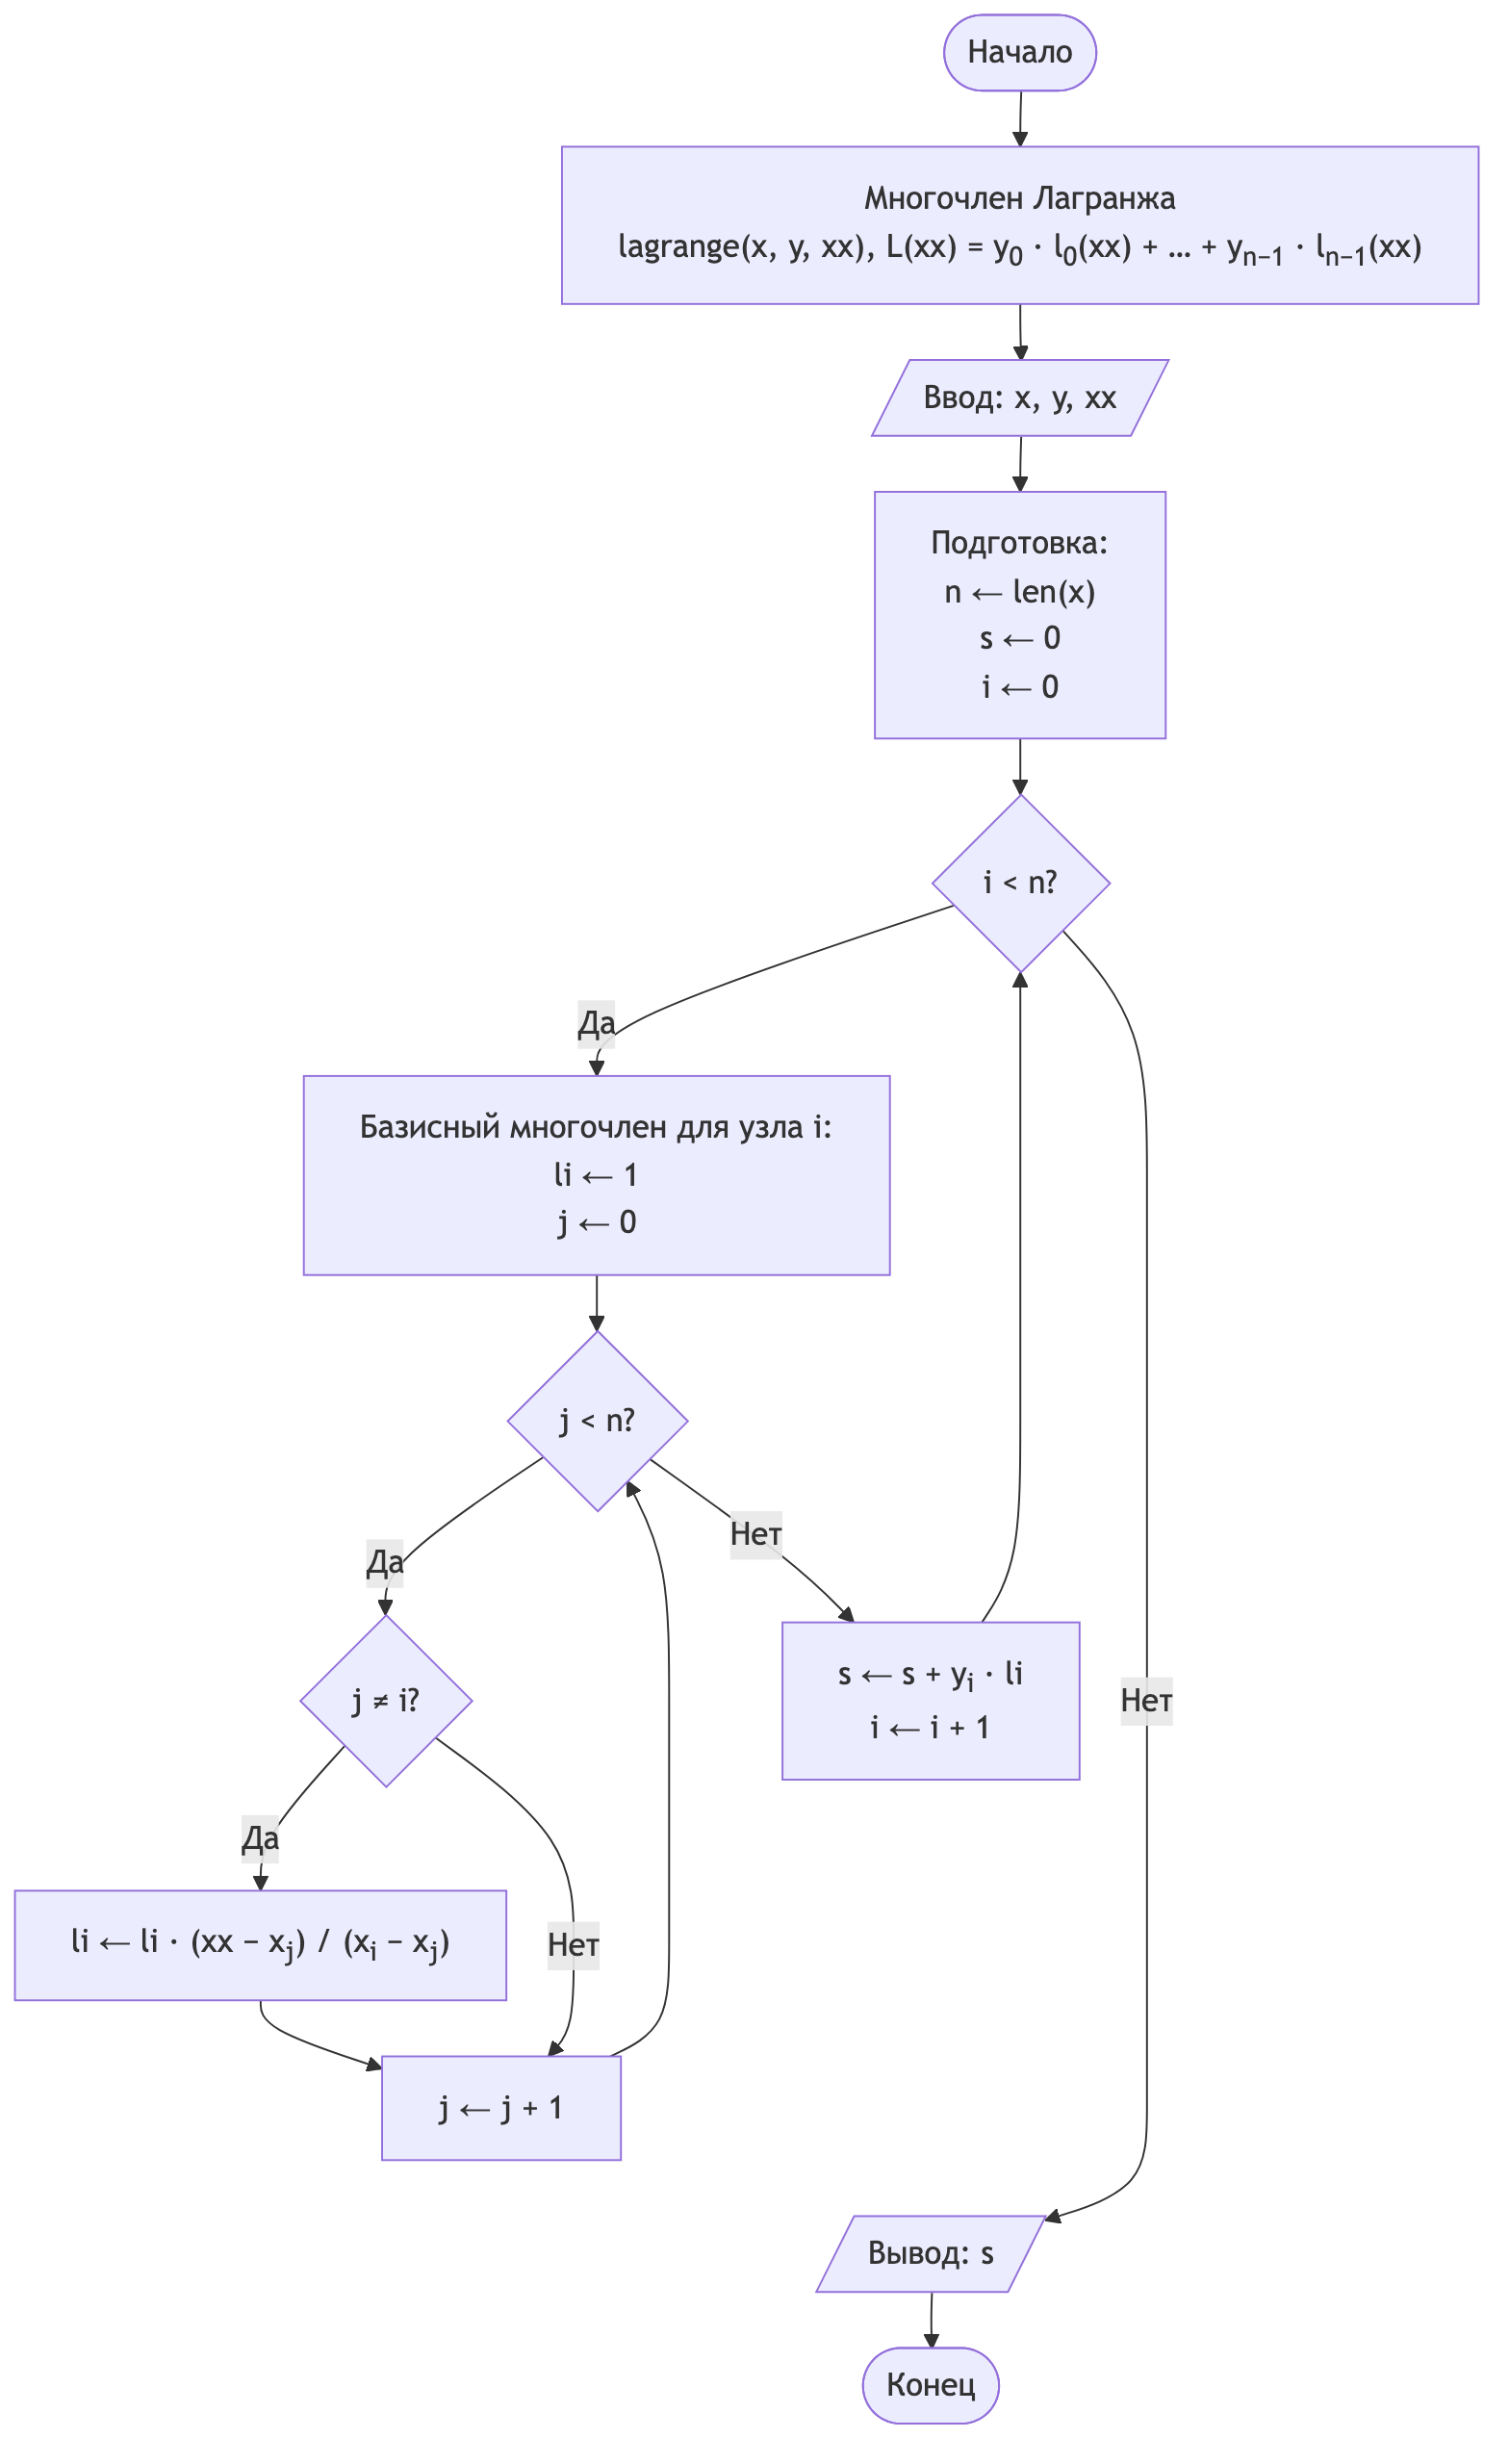
\includegraphics[width=\textwidth,height=0.82\textheight,keepaspectratio]{report_assets/lagrange.png}
    \caption{Блок-схема многочлена Лагранжа (функция \texttt{lagrange})}
\end{figure}

\begin{figure}[H]
    \centering
    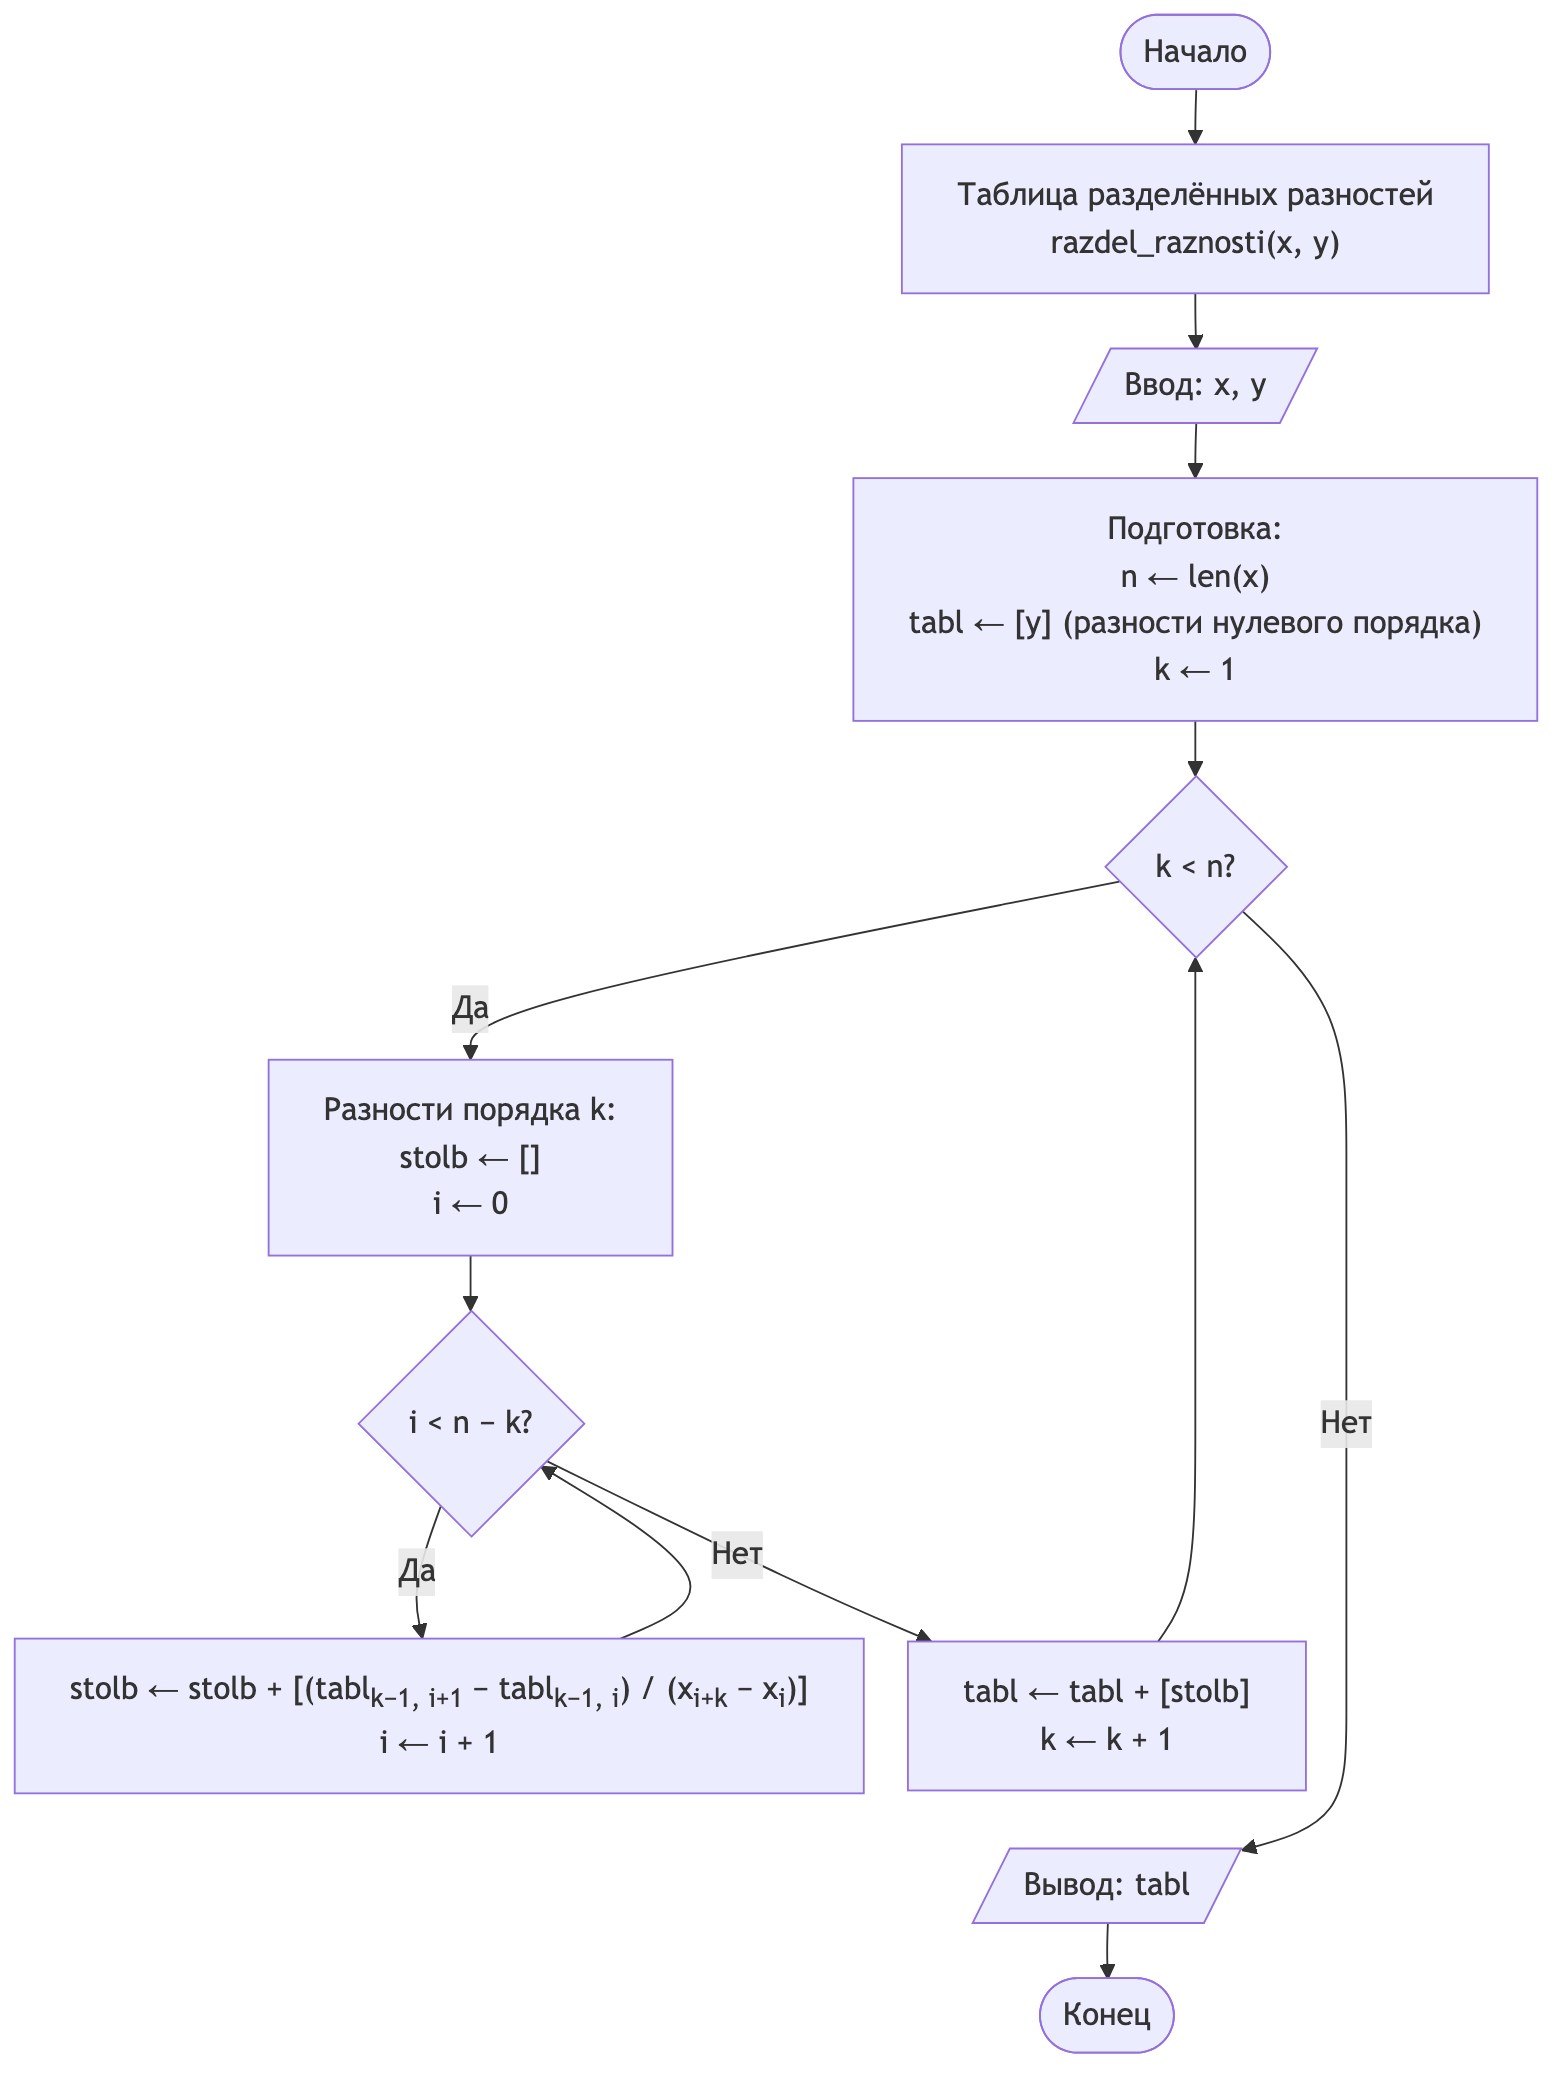
\includegraphics[width=\textwidth,height=0.82\textheight,keepaspectratio]{report_assets/razdel_raznosti.png}
    \caption{Блок-схема построения таблицы разделённых разностей (функция \texttt{razdel\_raznosti})}
\end{figure}

\begin{figure}[H]
    \centering
    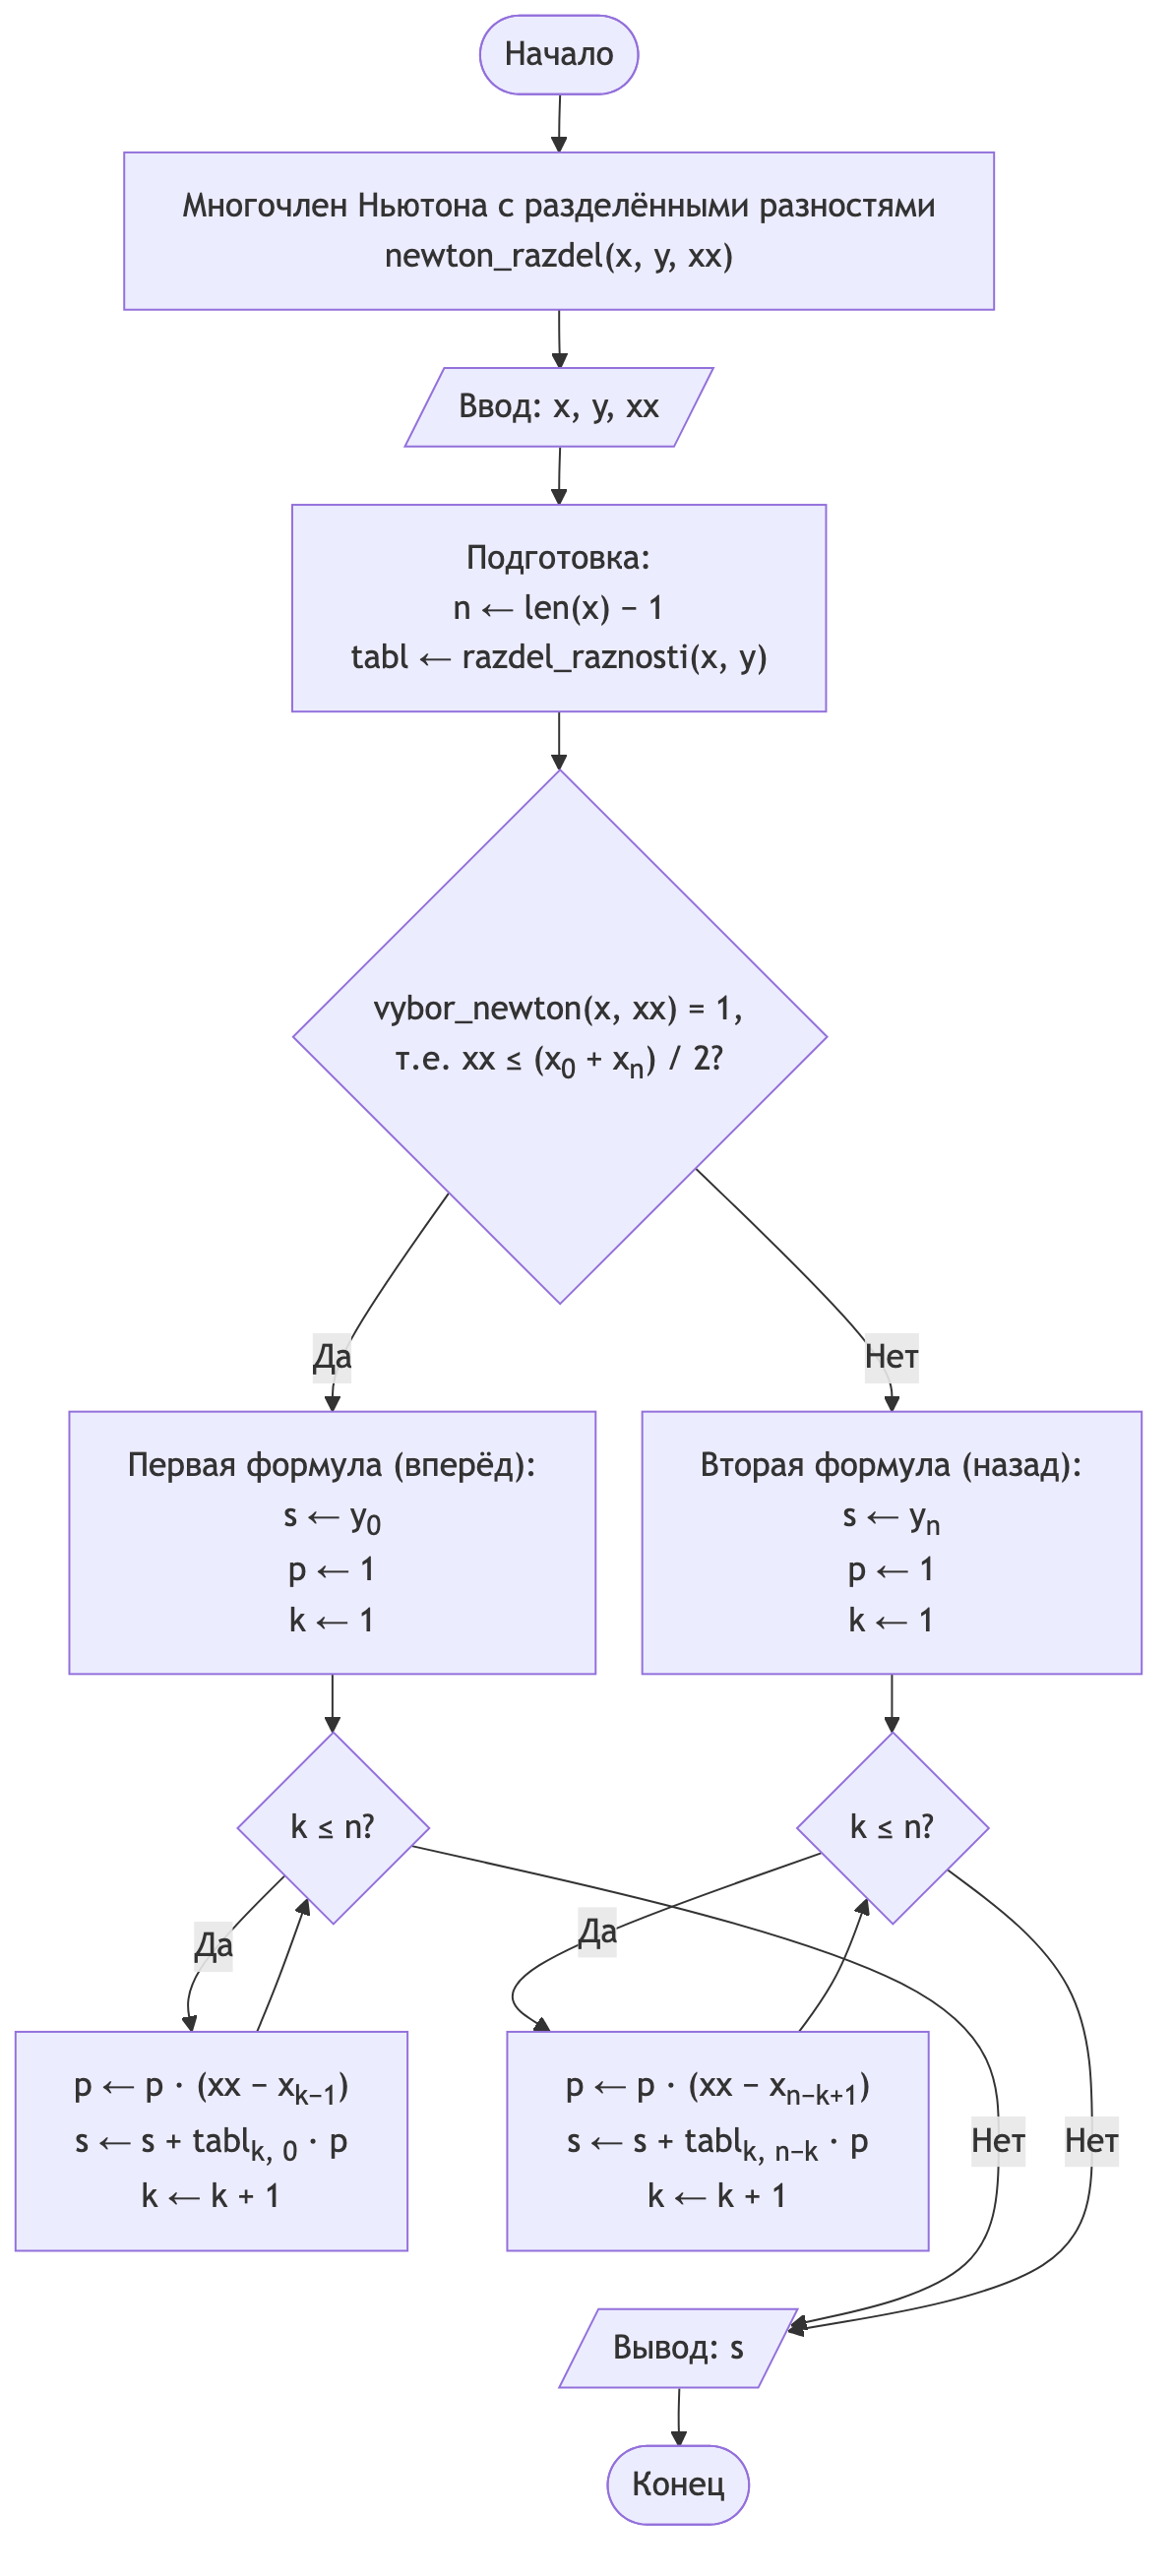
\includegraphics[width=\textwidth,height=0.82\textheight,keepaspectratio]{report_assets/newton_razdel.png}
    \caption{Блок-схема многочлена Ньютона с разделёнными разностями (функция \texttt{newton\_razdel})}
\end{figure}

\begin{figure}[H]
    \centering
    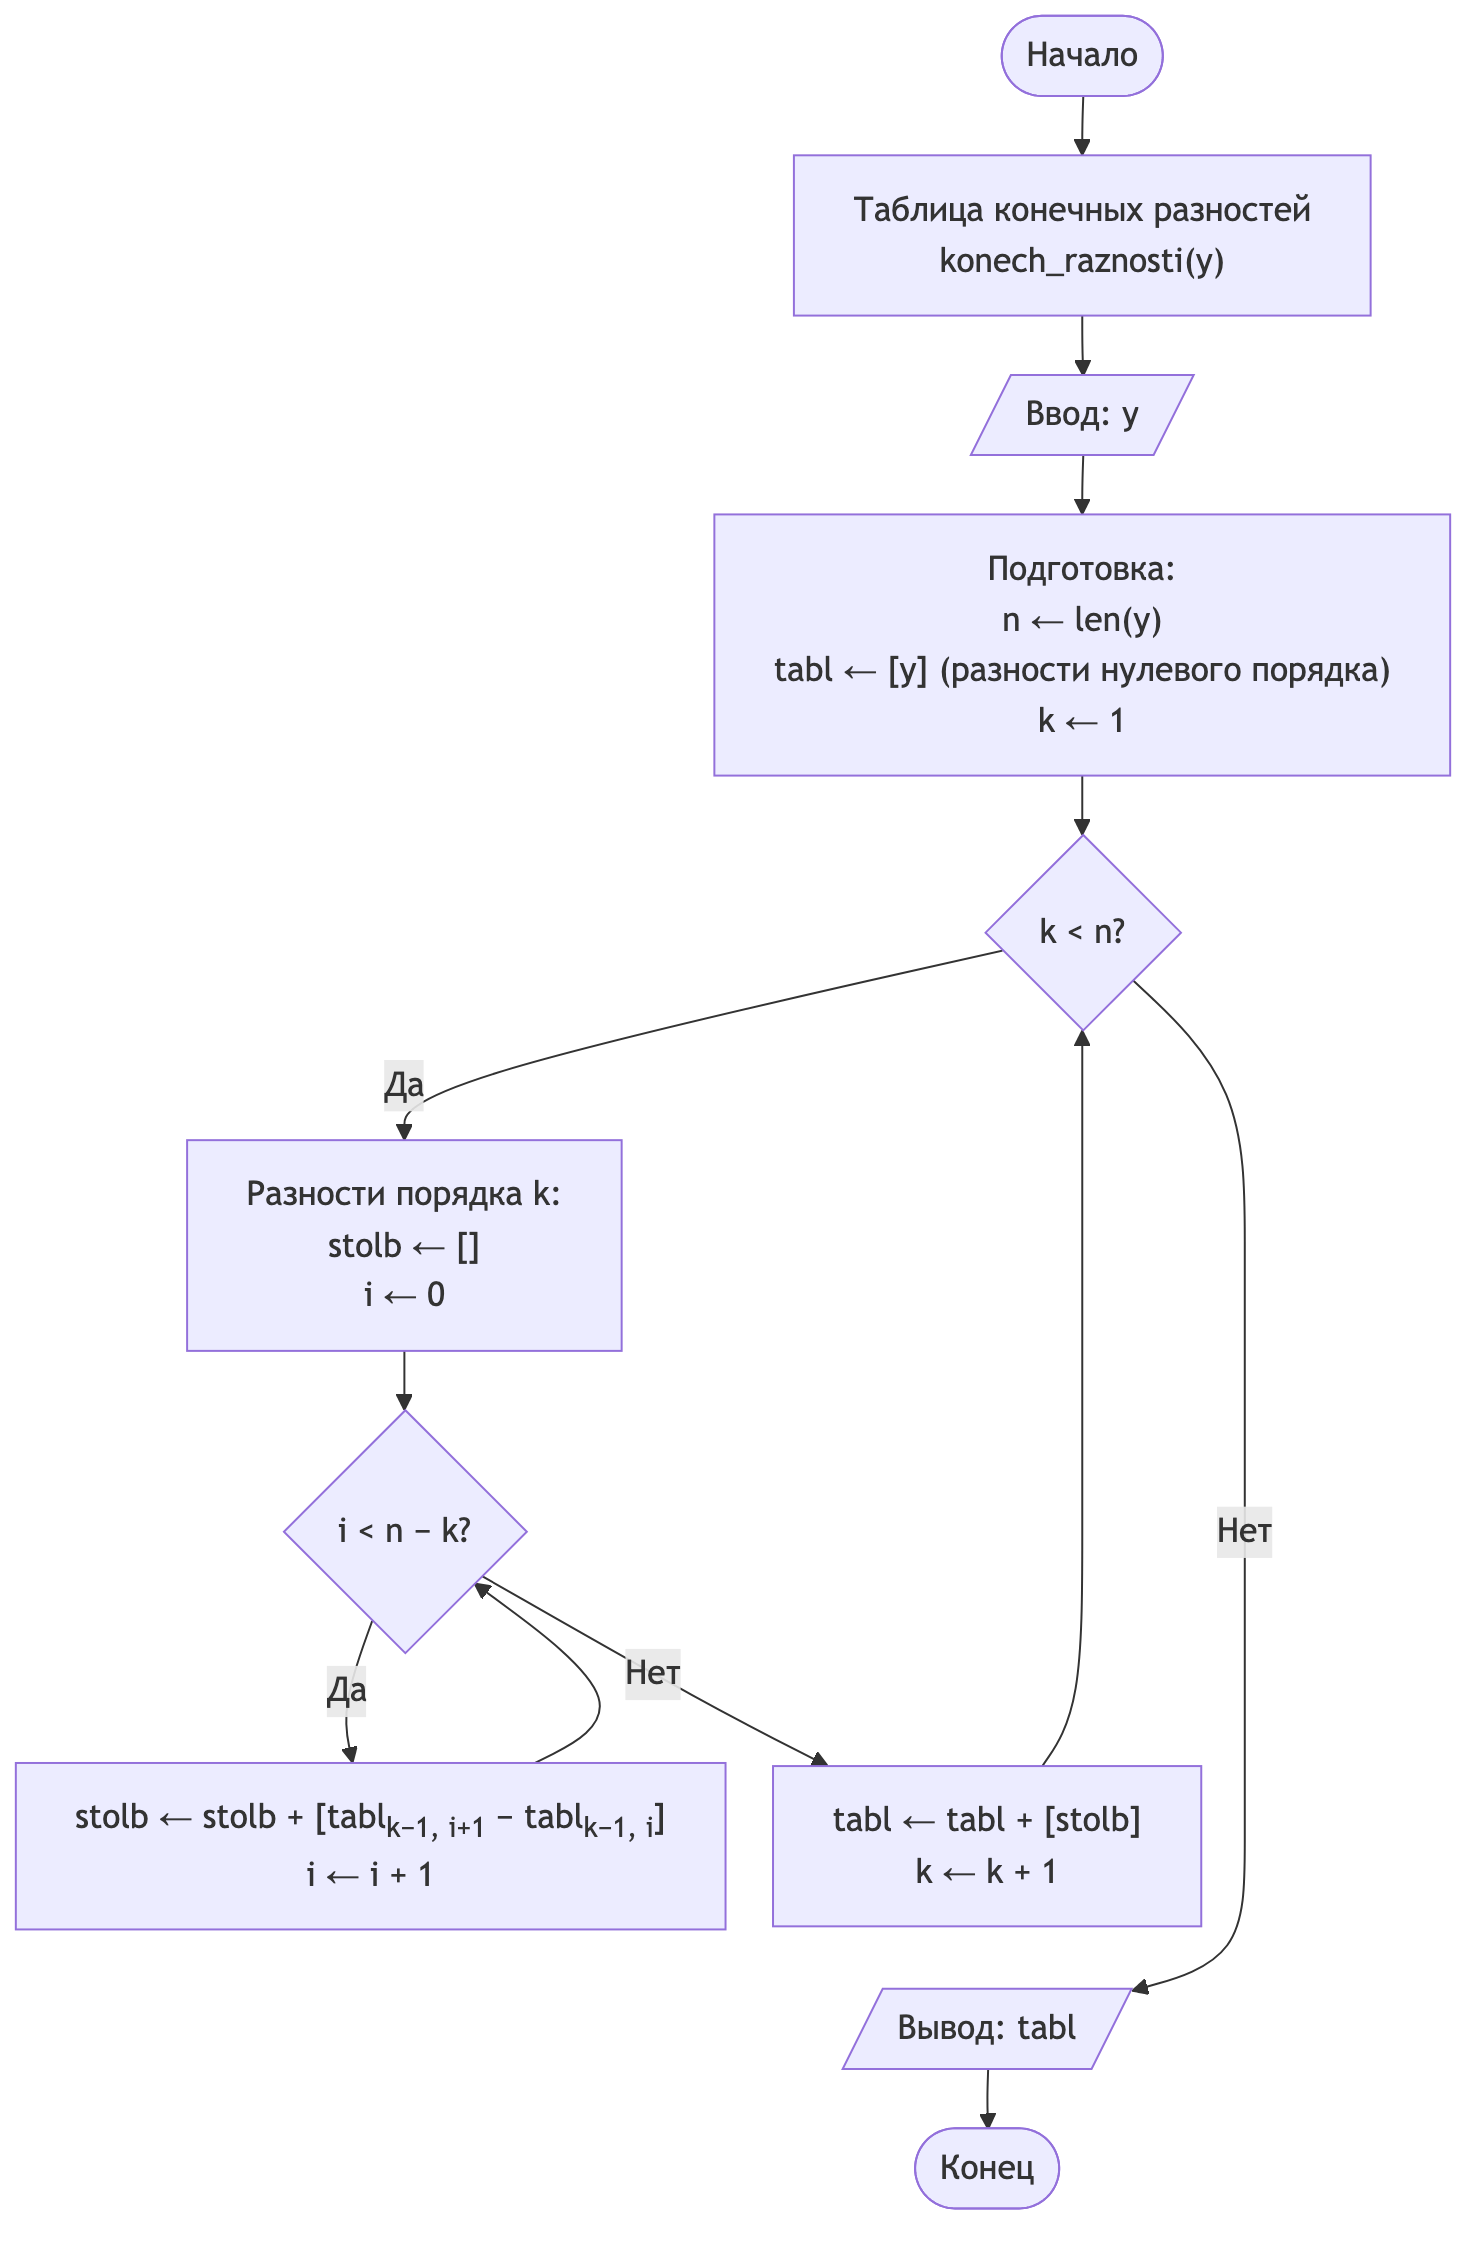
\includegraphics[width=\textwidth,height=0.82\textheight,keepaspectratio]{report_assets/konech_raznosti.png}
    \caption{Блок-схема построения таблицы конечных разностей (функция \texttt{konech\_raznosti})}
\end{figure}

\begin{figure}[H]
    \centering
    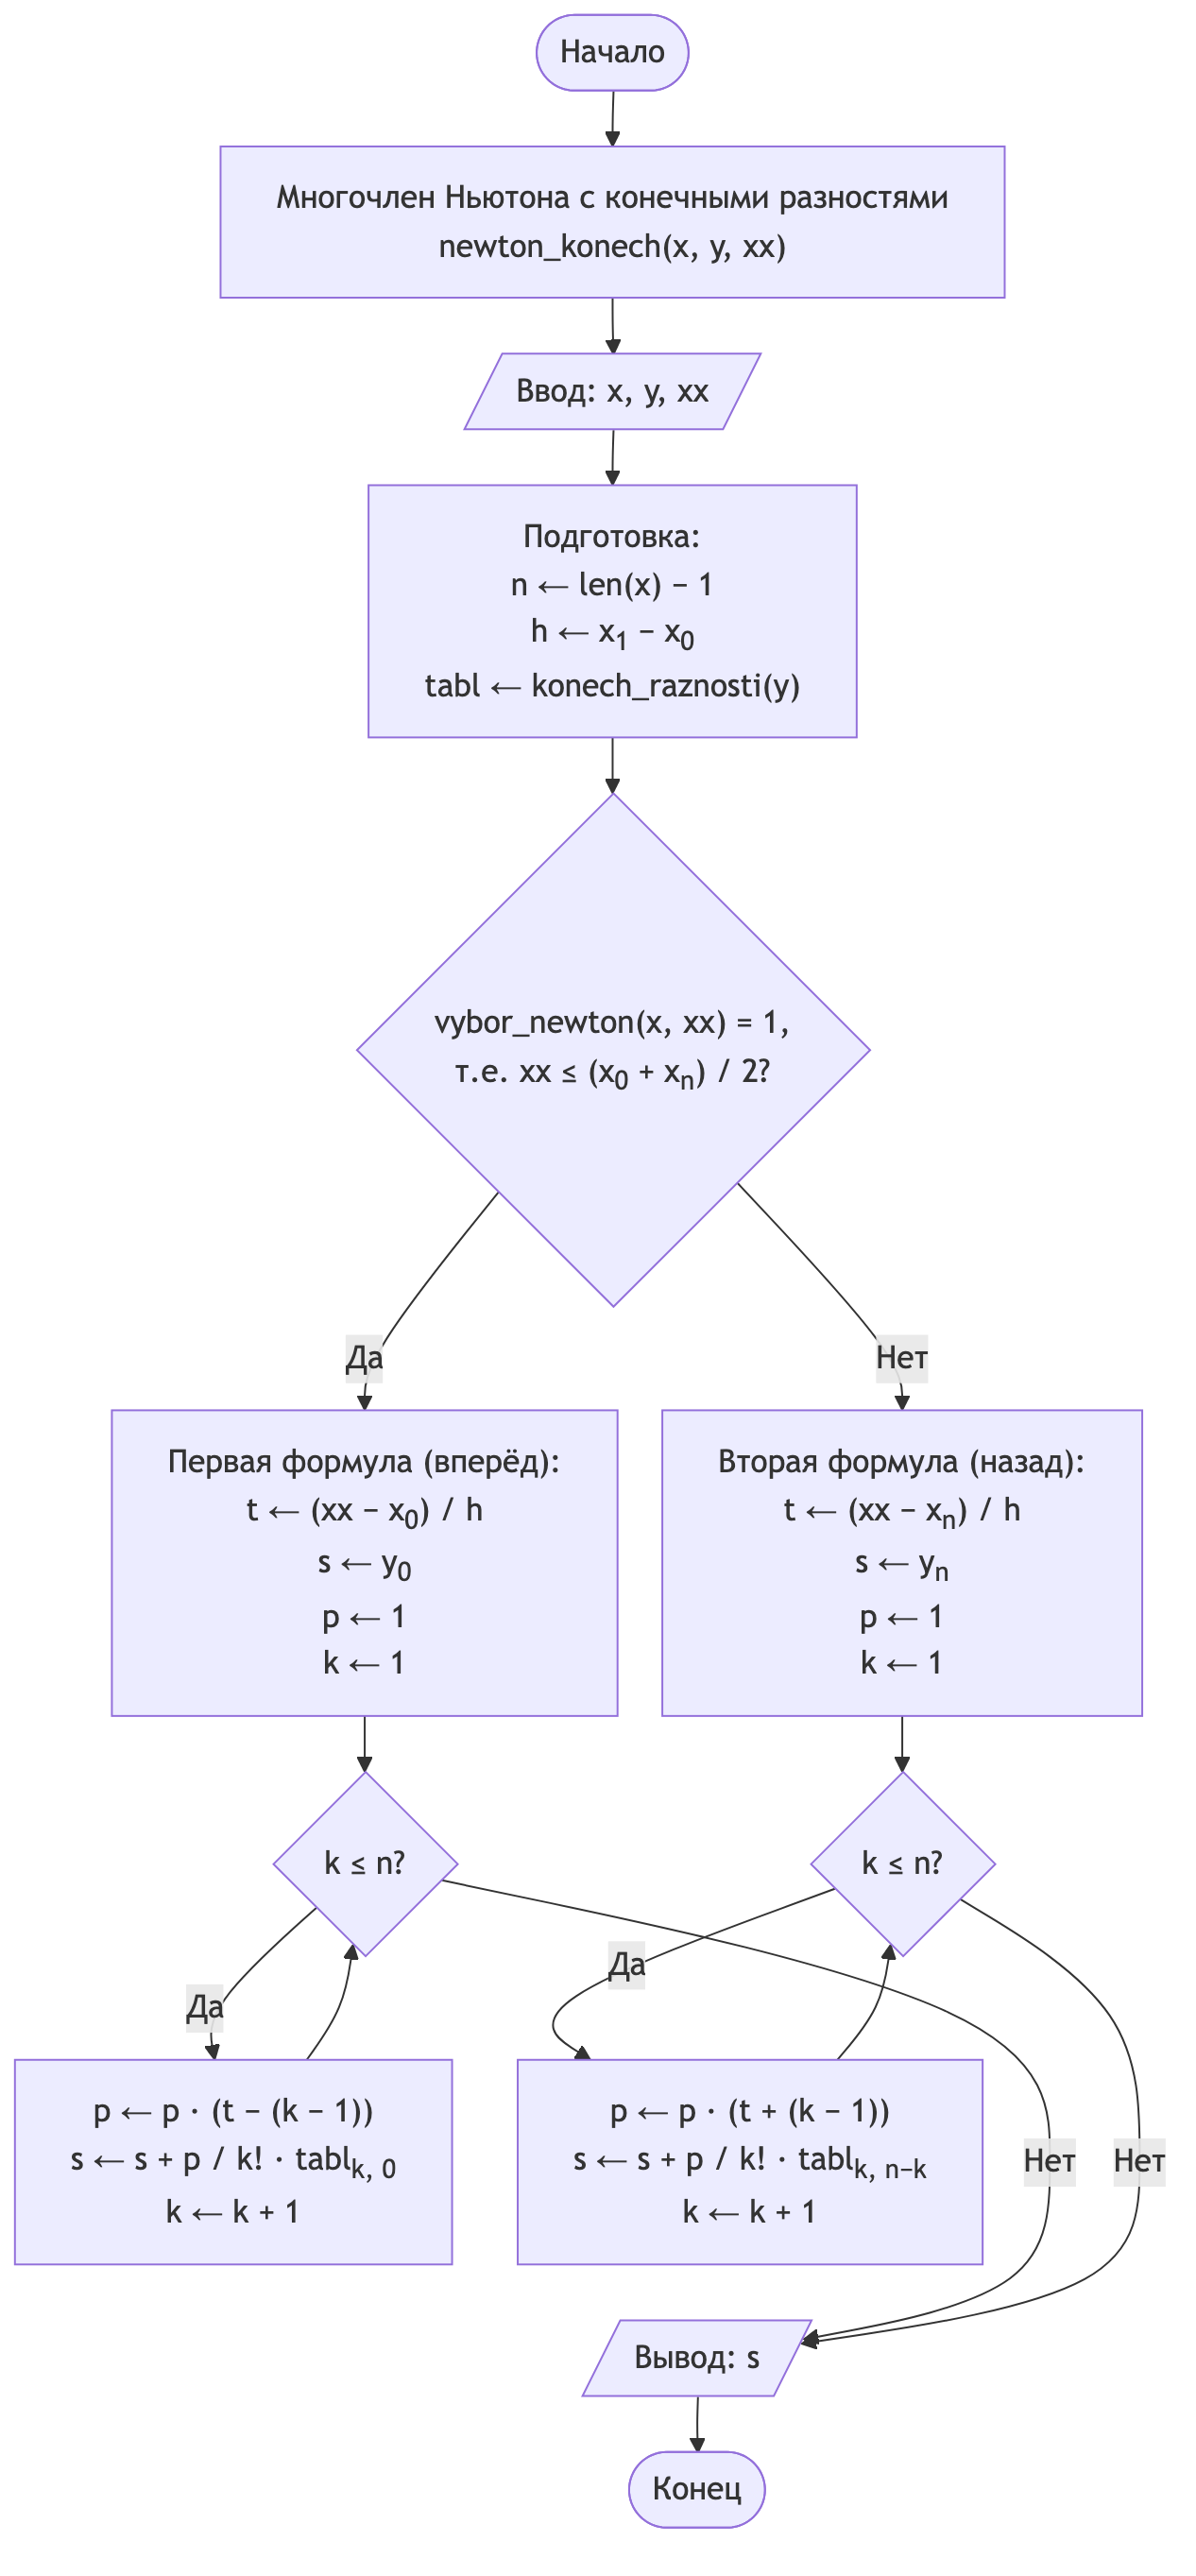
\includegraphics[width=\textwidth,height=0.82\textheight,keepaspectratio]{report_assets/newton_konech.png}
    \caption{Блок-схема многочлена Ньютона с конечными разностями (функция \texttt{newton\_konech})}
\end{figure}

\section*{Реализация численного метода}
Интерполяционные формулы реализованы в модуле \texttt{numerical.py}, проверки данных, выбор формулы и таблицы разностей -- в \texttt{interpolation.py} и \texttt{methods.py}, разбор введённого пользователем выражения $f(x)$ -- в \texttt{expression\_parser.py} (библиотека \texttt{sympy}), интерфейс -- в \texttt{app.py} и \texttt{plotting.py}. Ниже приведён код функций \texttt{numerical.py}.

\subsection*{Многочлен Лагранжа}
\begin{lstlisting}[language=Python,caption={Функция \texttt{lagrange}}]
def lagrange(x, y, xx):
    n = len(x)
    s = 0
    for i in range(n):
        li = 1
        for j in range(n):
            if j != i:
                li *= (xx - x[j]) / (x[i] - x[j])
        s += y[i] * li
    return s
\end{lstlisting}

\subsection*{Таблица разделённых разностей}
\begin{lstlisting}[language=Python,caption={Функция \texttt{razdel\_raznosti}}]
def razdel_raznosti(x, y):
    n = len(x)
    tabl = [list(y)]
    for k in range(1, n):
        stolb = []
        for i in range(n - k):
            stolb.append((tabl[k - 1][i + 1] - tabl[k - 1][i]) / (x[i + k] - x[i]))
        tabl.append(stolb)
    return tabl
\end{lstlisting}

\subsection*{Таблица конечных разностей}
\begin{lstlisting}[language=Python,caption={Функция \texttt{konech\_raznosti}}]
def konech_raznosti(y):
    n = len(y)
    tabl = [list(y)]
    for k in range(1, n):
        stolb = []
        for i in range(n - k):
            stolb.append(tabl[k - 1][i + 1] - tabl[k - 1][i])
        tabl.append(stolb)
    return tabl
\end{lstlisting}

\subsection*{Выбор формулы Ньютона}
\begin{lstlisting}[language=Python,caption={Функция \texttt{vybor\_newton}}]
def vybor_newton(x, xx):
    n = len(x) - 1
    if xx <= (x[0] + x[n]) / 2:
        return 1
    return 2
\end{lstlisting}

\subsection*{Многочлен Ньютона с разделёнными разностями}
\begin{lstlisting}[language=Python,caption={Функция \texttt{newton\_razdel}}]
def newton_razdel(x, y, xx):
    n = len(x) - 1
    tabl = razdel_raznosti(x, y)
    if vybor_newton(x, xx) == 1:
        s = y[0]
        p = 1
        for k in range(1, n + 1):
            p *= xx - x[k - 1]
            s += tabl[k][0] * p
    else:
        s = y[n]
        p = 1
        for k in range(1, n + 1):
            p *= xx - x[n - k + 1]
            s += tabl[k][n - k] * p
    return s
\end{lstlisting}

\subsection*{Многочлен Ньютона с конечными разностями}
\begin{lstlisting}[language=Python,caption={Функция \texttt{newton\_konech}}]
def newton_konech(x, y, xx):
    n = len(x) - 1
    h = x[1] - x[0]
    tabl = konech_raznosti(y)
    if vybor_newton(x, xx) == 1:
        t = (xx - x[0]) / h
        s = y[0]
        p = 1
        for k in range(1, n + 1):
            p *= t - (k - 1)
            s += p / math.factorial(k) * tabl[k][0]
    else:
        t = (xx - x[n]) / h
        s = y[n]
        p = 1
        for k in range(1, n + 1):
            p *= t + (k - 1)
            s += p / math.factorial(k) * tabl[k][n - k]
    return s


if __name__ == "__main__":
    x = [0.1, 0.2, 0.3, 0.4, 0.5]
    y = [1.25, 2.38, 3.79, 5.44, 7.14]
    print(lagrange(x, y, 0.35))
    print(newton_konech(x, y, 0.15), newton_konech(x, y, 0.47))
    print(newton_razdel([0.15, 0.2, 0.33, 0.47], [1.25, 2.38, 3.79, 5.44], 0.22))
    for stroka in konech_raznosti(y):
        print(stroka)
\end{lstlisting}

\section*{Пример работы}
Узлы вводятся в таблицу вручную, кликом по графику, из файла или формируются табулированием функции на отрезке $[a;b]$ по $n$ узлам. Функция задаётся выражением через $x$ (по умолчанию \texttt{sin(x)}), например \texttt{cos(x)}, \texttt{exp(-x\^{}2)} или \texttt{x*sin(x)}; поддерживаются \texttt{sin}, \texttt{cos}, \texttt{tg}, \texttt{exp}, \texttt{ln}, \texttt{sqrt}, \texttt{abs}, степени и константы $e$, $\pi$. Десятичный разделитель везде -- точка или запятая, значения выводятся без ограничения числа знаков. Точка интерполяции $x$ вводится в отдельное поле. Для загрузки из файла подготовлены тестовые наборы в каталоге \texttt{examples}: \texttt{variant4.txt}, \texttt{lecture\_uniform.txt}, \texttt{lecture\_divided.txt}, а также некорректные \texttt{invalid\_duplicate.txt} и \texttt{invalid\_format.txt}. Таблицы конечных и разделённых разностей строятся сразу при вводе узлов, расчёт значения выполняется всеми тремя методами, а флажки управляют тем, какие кривые показаны на графике.

\subsection*{Набор 1: таблица варианта 4}
Для семи узлов таблицы 1.4 и точки $x=1{,}051$ программа получает:
\begin{quote}
    Узлы равноотстоящие, $h=0{,}1$; точка внутри отрезка $[1{,}05;1{,}65]$. Многочлен Лагранжа: $P(1{,}051)=0{,}13167182$. Ньютон, разделённые разности: первая формула (вперёд), $P(1{,}051)=0{,}13167182$. Ньютон, конечные разности: первая формула (вперёд), $t=0{,}01$, $P(1{,}051)=0{,}13167182$. Разброс между методами $8{,}3\cdot10^{-17}$.
\end{quote}
Результат совпадает со значением, полученным в вычислительной части. Для $x=1{,}277$ программа даёт $P(1{,}277)=2{,}42028592$, что совпадает со значением по формуле Гаусса.

\begin{figure}[H]
    \centering
    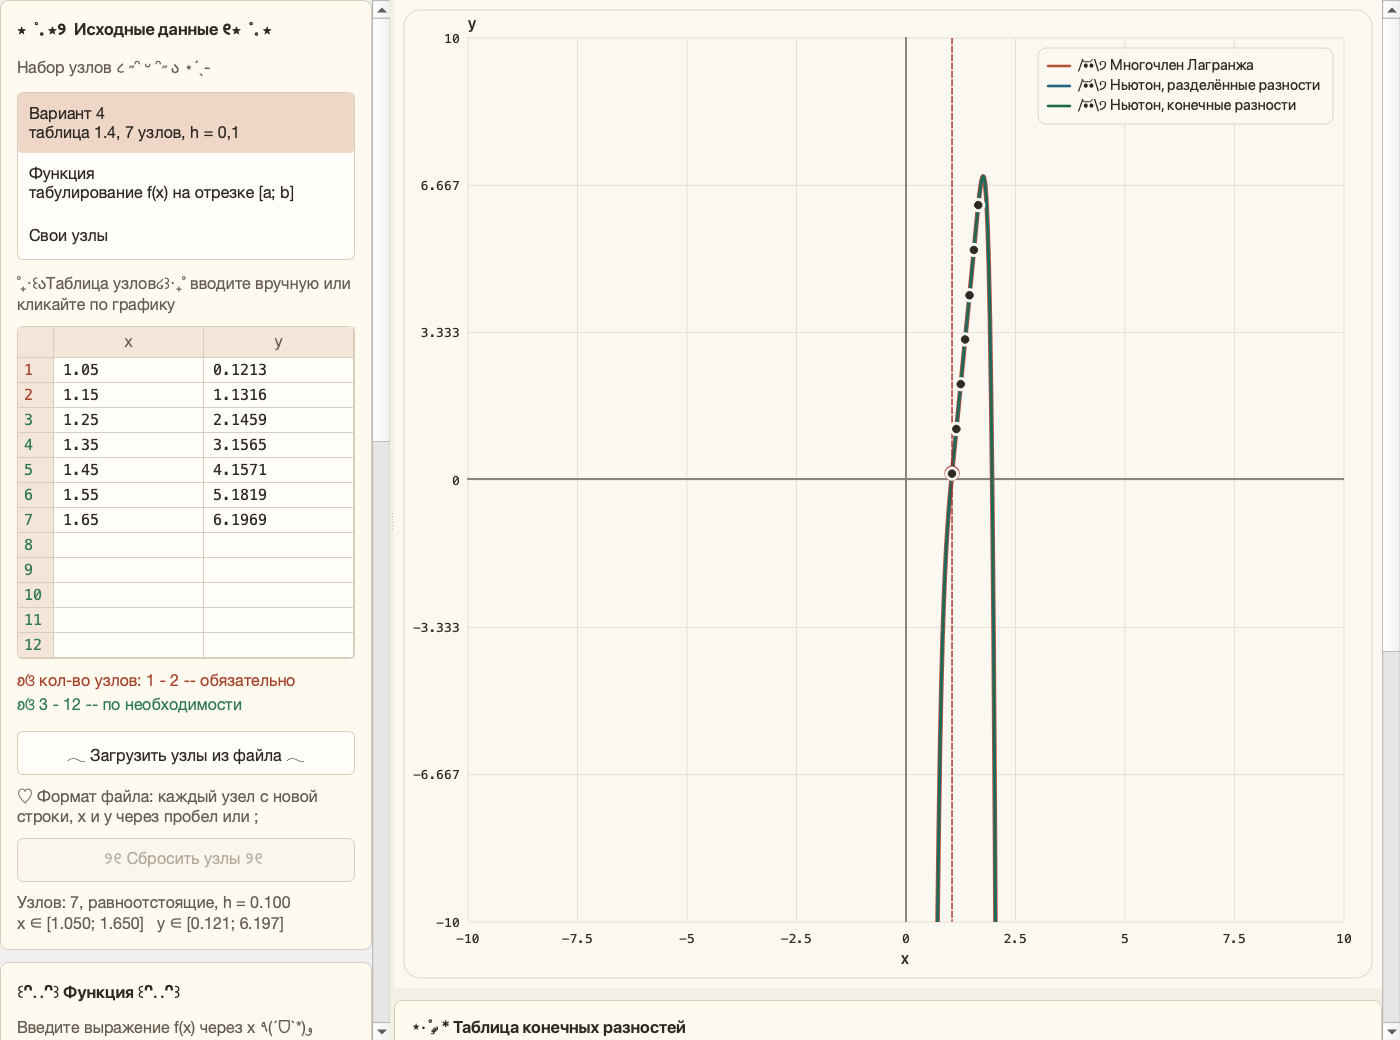
\includegraphics[width=\textwidth]{report_assets/screenshot_variant4.png}
    \caption{Пример работы программы для таблицы варианта 4}
\end{figure}

\begin{figure}[H]
    \centering
    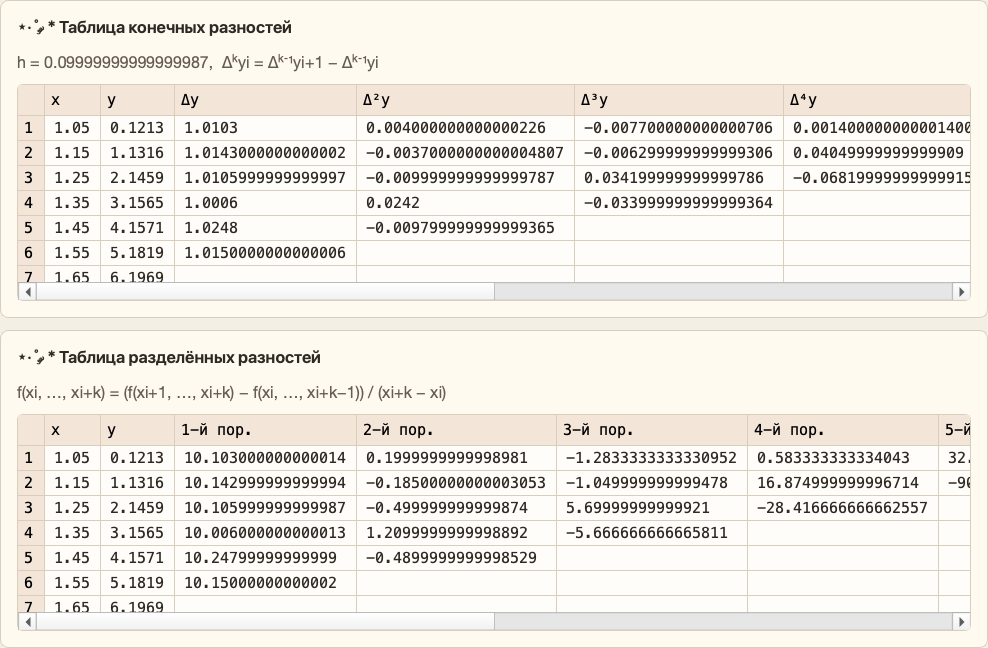
\includegraphics[width=\textwidth]{report_assets/tables_variant4.png}
    \caption{Таблицы конечных и разделённых разностей для таблицы варианта 4}
\end{figure}

\subsection*{Набор 2: функция, заданная выражением}
Узлы получены табулированием $f(x)=\sin x$ на отрезке $[0;3]$ по 7 узлам ($h=0{,}5$), точка $x=1{,}3$:
\begin{quote}
    Все три метода дают $P(1{,}3)=0{,}96355980$, точное значение $\sin1{,}3=0{,}96355819$, погрешность $|P-f|=1{,}6\cdot10^{-6}$.
\end{quote}
На графике исходная функция показана пунктиром, интерполяционные многочлены -- сплошными линиями.

\begin{figure}[H]
    \centering
    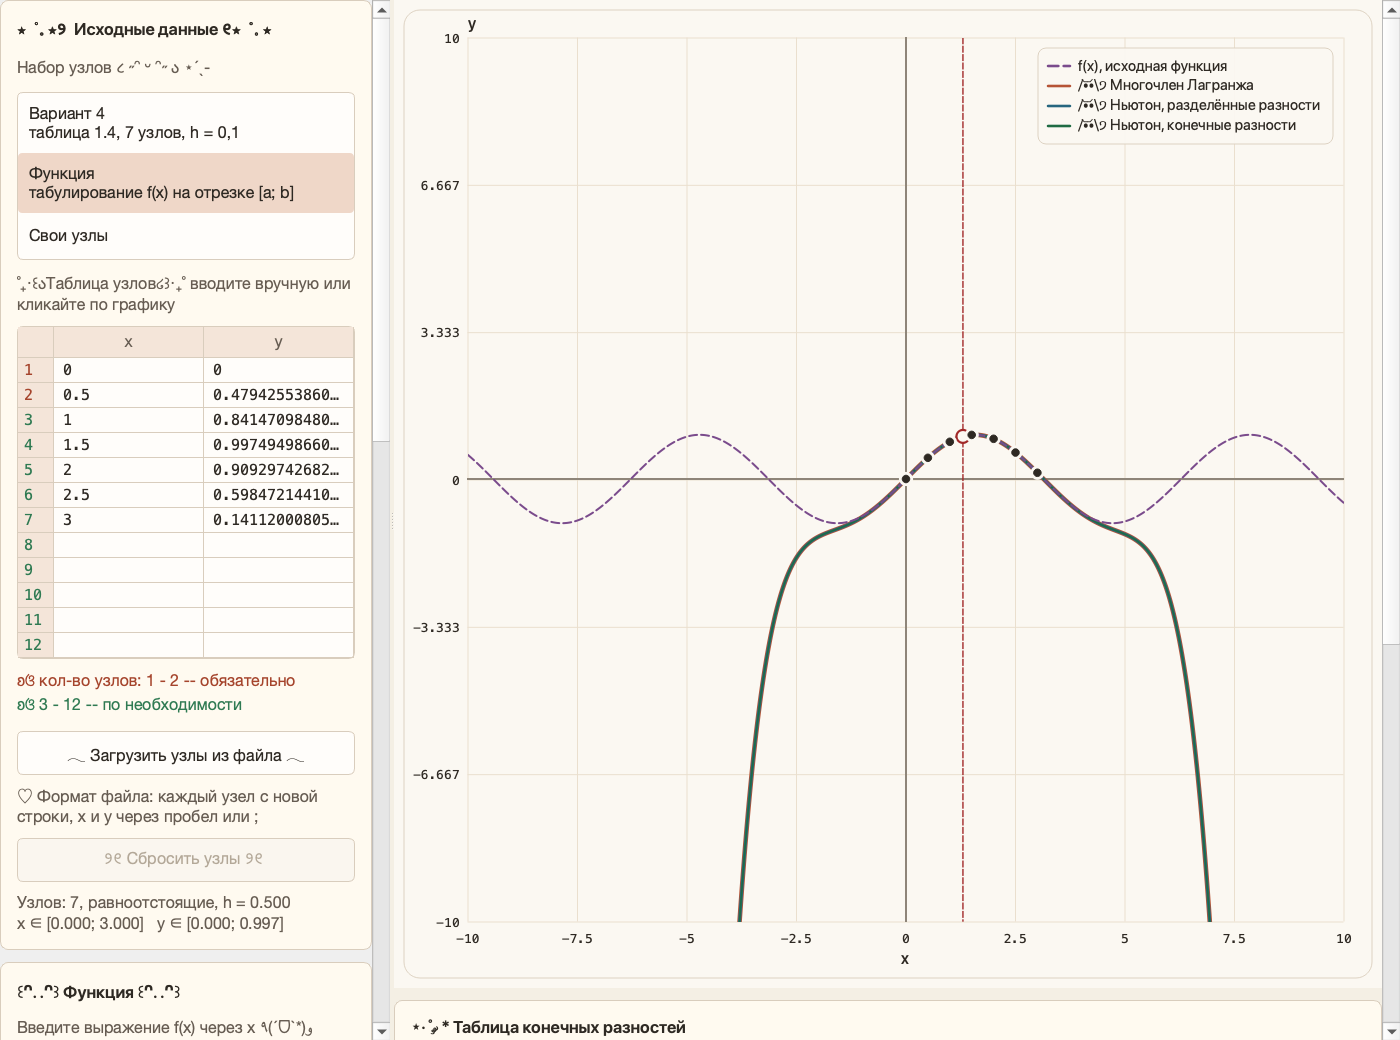
\includegraphics[width=\textwidth]{report_assets/screenshot_function.png}
    \caption{Пример работы программы при табулировании функции $\sin x$}
\end{figure}

Для выражения $f(x)=x\sin x$ на том же отрезке программа получает $P(1{,}3)=1{,}25274$ при точном значении $f(1{,}3)=1{,}25263$, погрешность $1{,}2\cdot10^{-4}$; при ошибке в выражении (посторонняя переменная, незакрытая скобка, деление на ноль в узле) таблица не заполняется и выводится сообщение о причине.

\begin{figure}[H]
    \centering
    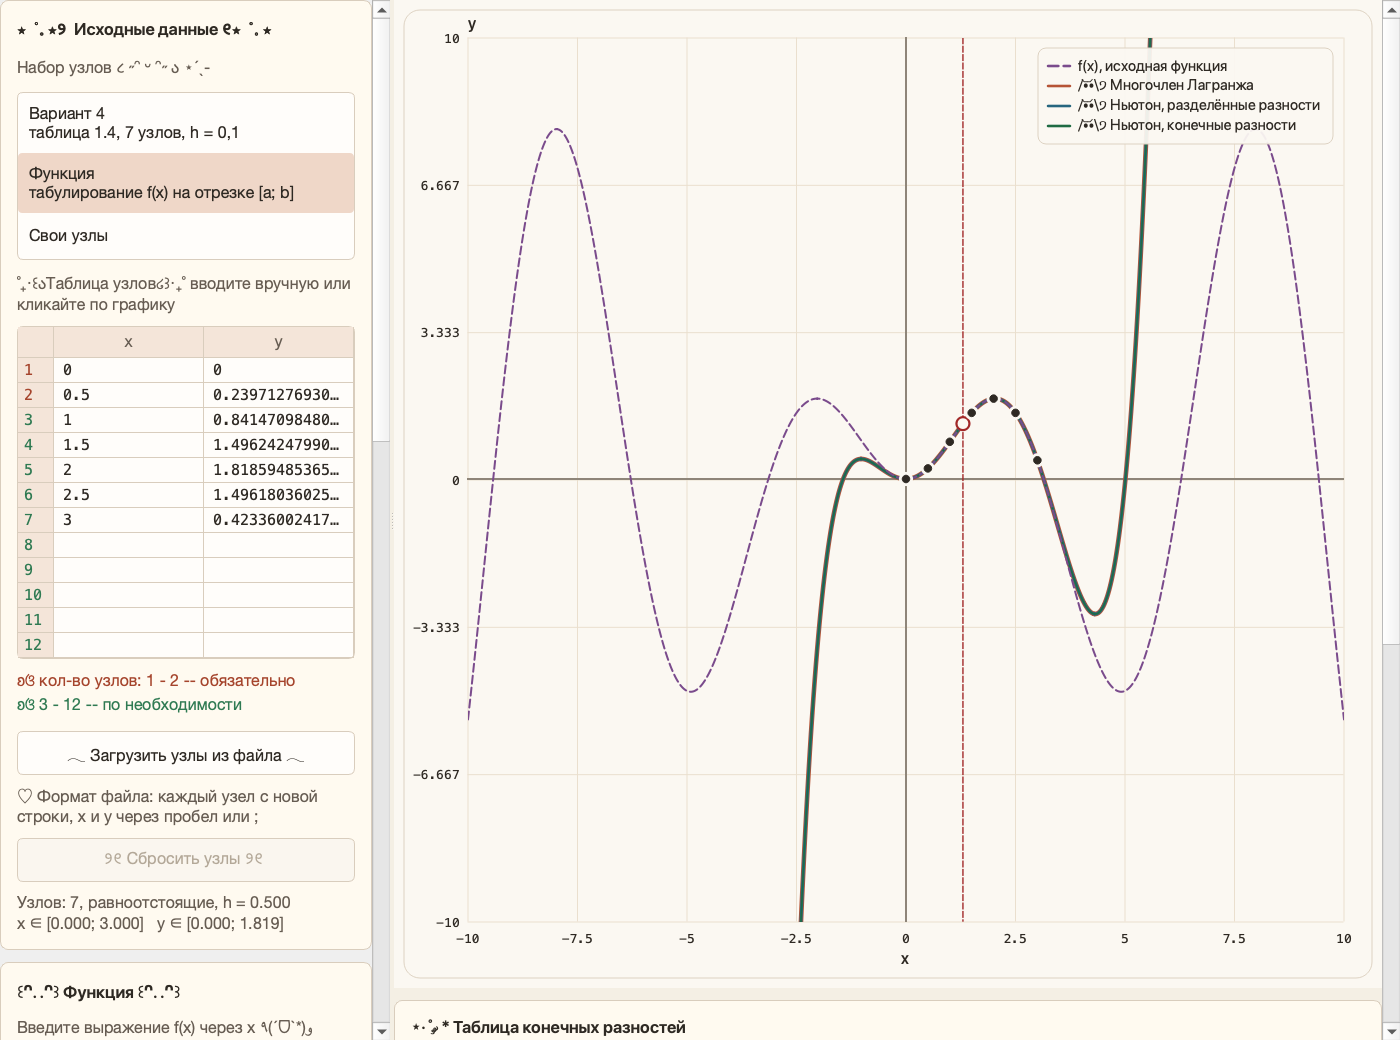
\includegraphics[width=\textwidth]{report_assets/screenshot_custom.png}
    \caption{Пример работы программы для введённого выражения $x\sin x$}
\end{figure}

\subsection*{Набор 3: неравноотстоящие узлы и некорректные данные}
Для узлов $0{,}15$; $0{,}2$; $0{,}33$; $0{,}47$ (пример из лекции, загружен из файла \texttt{lecture\_divided.txt}) и точки $x=0{,}22$ многочлен Лагранжа и многочлен Ньютона с разделёнными разностями дают $P(0{,}22)=2{,}70748130$ (в лекции $2{,}70748$), а метод конечных разностей не применяется:
\begin{quote}
    <<не вычислен: узлы не равноотстоящие, конечные разности не применимы>>.
\end{quote}

\begin{figure}[H]
    \centering
    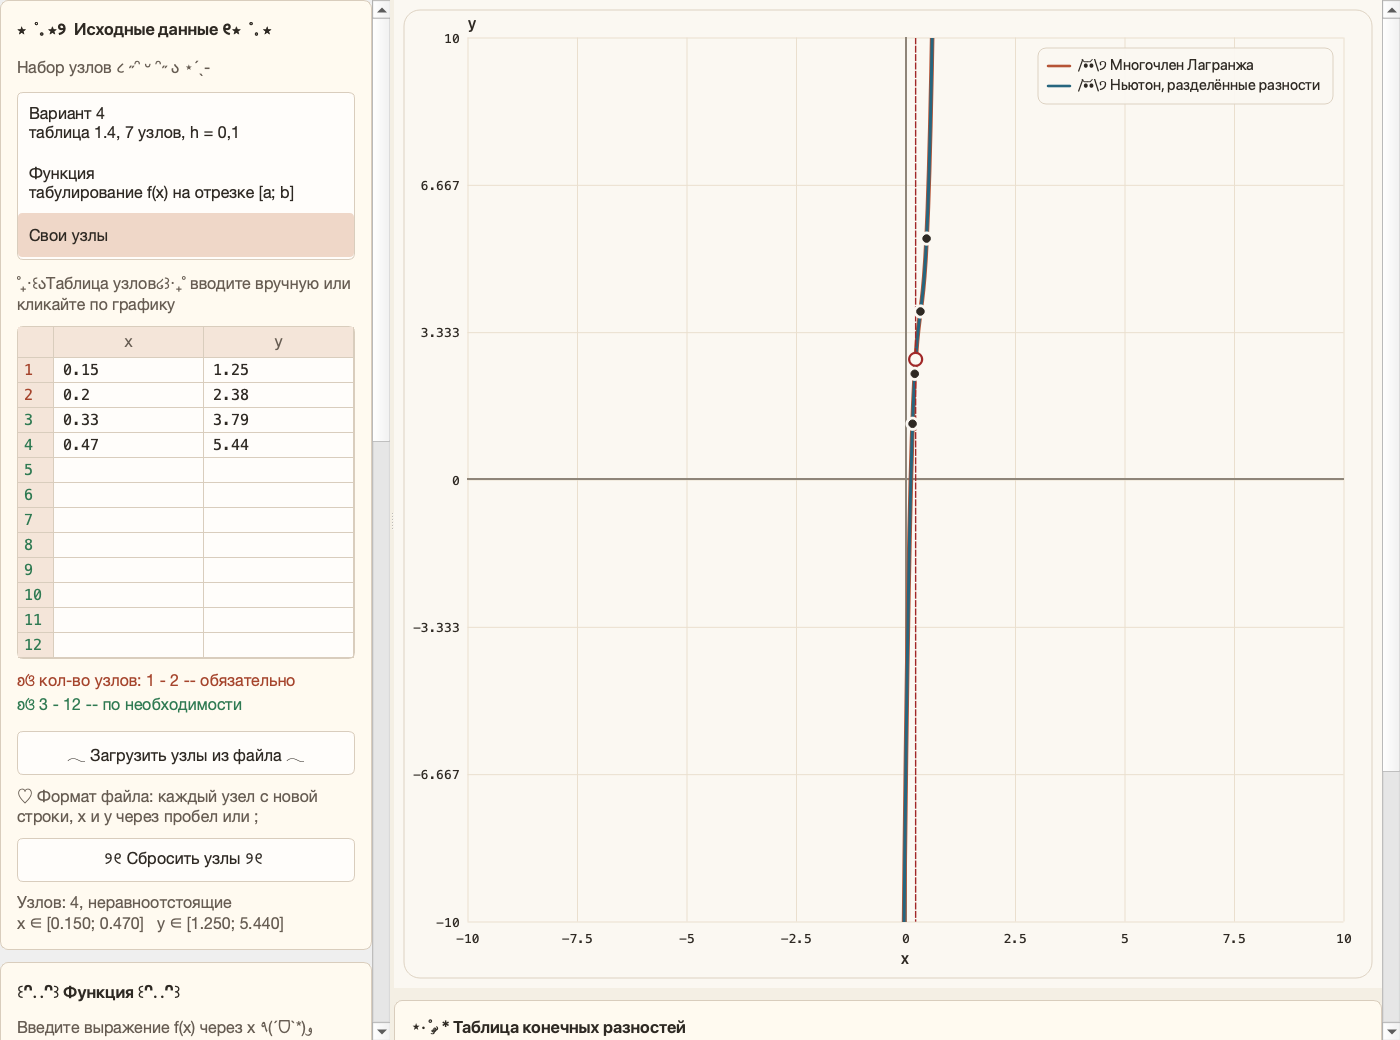
\includegraphics[width=\textwidth]{report_assets/screenshot_divided.png}
    \caption{Пример работы программы при неравноотстоящих узлах, загруженных из файла}
\end{figure}

Если два узла имеют одинаковый $x$, расчёт не выполняется:
\begin{quote}
    <<Узлы интерполяции должны быть различны: x = 2 повторяется.>>
\end{quote}
Если узлов меньше двух, больше двенадцати, поле $x$ не заполнено или содержит не число, программа также сообщает об ошибке, например:
\begin{quote}
    <<Нужно не меньше 2 узлов, введено 1.>>, <<Некорректное число в поле "x": abc. Используйте число с точкой или запятой.>>
\end{quote}
Если точка $x$ лежит вне отрезка $[x_0;x_n]$, значение вычисляется, но программа предупреждает об экстраполяции.

\begin{figure}[H]
    \centering
    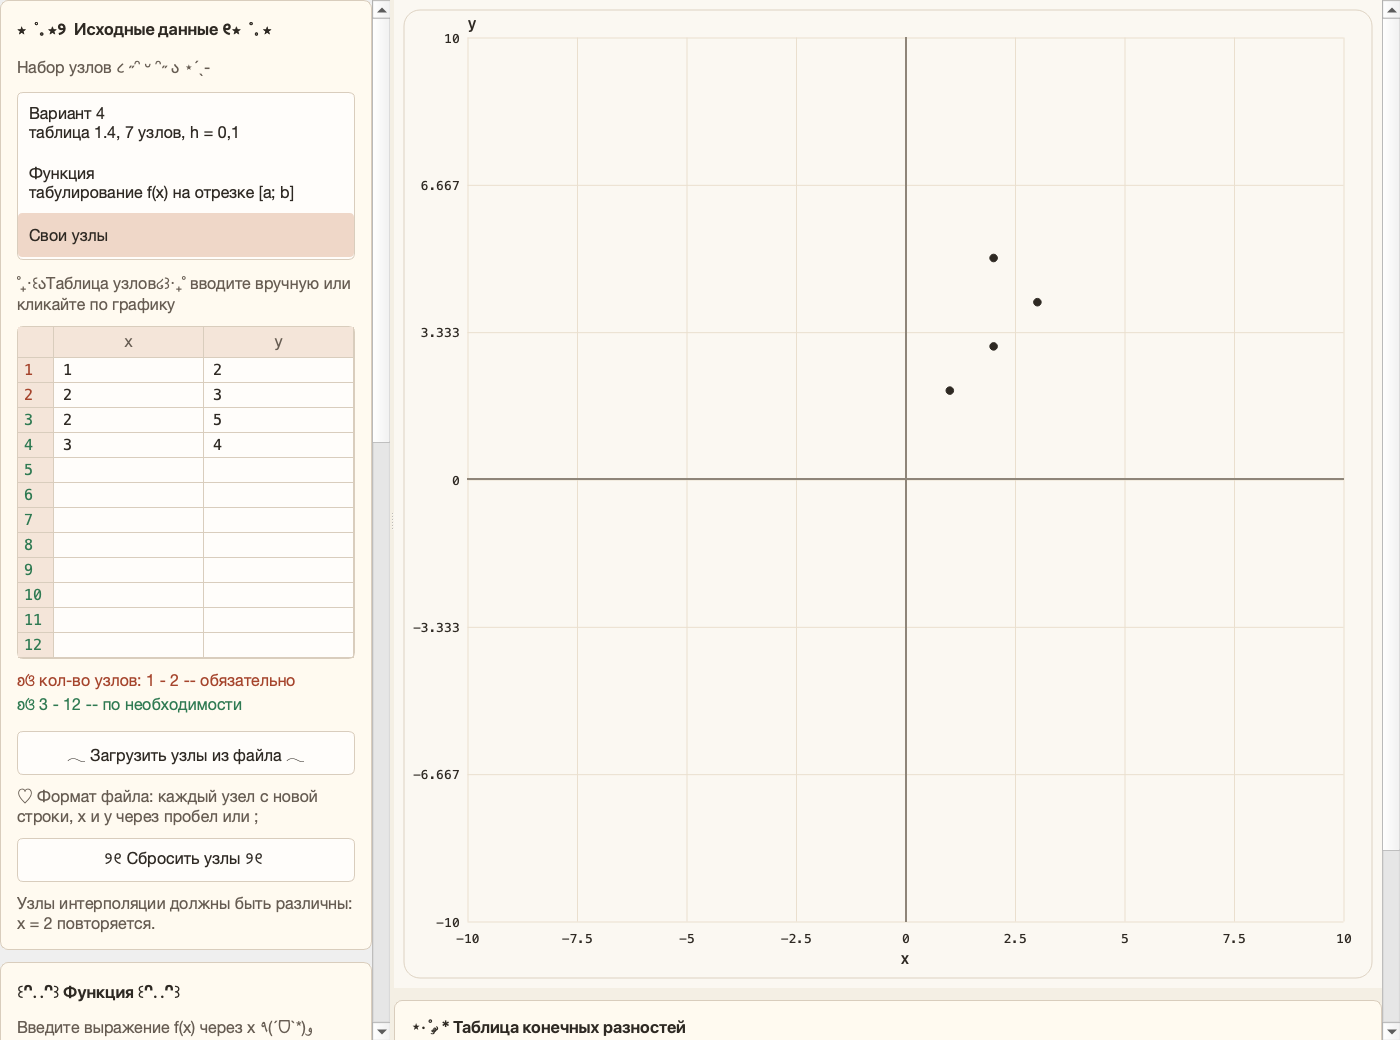
\includegraphics[width=\textwidth]{report_assets/screenshot_invalid.png}
    \caption{Реакция программы на совпадающие узлы}
\end{figure}

\section*{Ссылка на GitHub}
\url{https://github.com/juliakrasnoshtanova/itmo_compmath_lab5}

\section*{Вывод}
Реализована программа интерполяции табличной функции многочленом Лагранжа и многочленами Ньютона с разделёнными и конечными разностями (первая и вторая формулы). Программа принимает узлы с клавиатуры, из файла или табулированием функции, заданной выражением, строит таблицы конечных и разделённых разностей, вычисляет значение в заданной точке всеми методами, сравнивает результаты и строит графики. Для варианта 4 в вычислительной части получено $y(1{,}051)\approx0{,}13167$ по первой формуле Ньютона и $y(1{,}277)\approx2{,}42029$ по второй формуле Гаусса; многочлен Лагранжа и программа дают те же значения, поскольку все формулы описывают один и тот же интерполяционный многочлен.

\end{document}
